This chapter will detail some fundamental mathematical theory, techniques for minimisations, discussion about the theory of retinotopic mapping and applications to more general optimisations problems such as the Travelling Salesman Problem, a review of existing models and their limitations, and the research questions which this thesis will address.
\section{Fundamental Mathematics}
Some useful mathematical results, definitions, and standard computational procedures used throughout the text will be covered before discussing details of modelling retinotopic systems. These shall be discussed in general and without formal proof. There are several foundational texts recommended for further discussion \cite{Korner1988-wt, Gelfand2000-xr, Ablowitz2003-iv, Goodfellow-et-al-2016}.
\subsection{Fourier Transform}
The Fourier transform is useful analysis tool which transforms a function into its frequency domain. This thesis will use the following definition of the Fourier transform $\hat{f}(k)$ of a function $f(x)$:
\begin{equation}
\hat{f}(k) = \frac{1}{\sqrt{2 \pi}} \int_{-\infty}^{\infty} e^{-i kx} f(x) dx
\end{equation}
with the inverse transform mapping back from the frequency domain being defined as:
\begin{equation}
f(x) = \frac{1}{\sqrt{2 \pi}} \int_{-\infty}^{\infty} e^{i kx} \hat{f}(k) dk.
\end{equation}
The operation is linear following from the linearity of integration allowing it to be distributed over functions which are compositions of functions. The transform is real if and only if the function on which it operates is a linear combination of even functions and analogously is imaginary if and only if the function is a linear combination of odd functions. The Fourier transform has several elegant algebraic properties which make it useful in differential equation analysis and for evaluating certain integrals.
\paragraph{Fourier Phase Shifting Property}
The Fourier shifting theorem relates the phase of a function to a rotation in the complex plane. The theorem statement is simply:
\begin{equation}
\mathcal{F}[f(x + \phi)] = e^{i \phi}\hat{f}(k).
\end{equation}

\paragraph{Fourier Scaling Property}
The Fourier transform is scaled in a straightforward manner:
\begin{equation}
\mathcal{F}[f(a x)] = \frac{1}{|c|}\hat{f}(\frac{k}{c}).
\end{equation}
\subsubsection{Fourier Convolution Theorem}
The Fourier convolution theorem allows for convolutions of functions to be decomposed into their products in Fourier space. It is stated as:
\begin{equation}
\mathcal{F}[(f\star g)(x)](k) = \sqrt{2 \pi}\hat{f}(k) \hat{g}(k),
\end{equation}
where $\star$ denotes the convolution operator: $(f \star g)(x) = \int_{-\infty}^{\infty} f(x-\xi)g(\xi) d \xi$.

\paragraph{Fourier Differentiation Operator}
The Fourier transform allows derivatives to be transformed into polynomial expressions:
\begin{equation}
\mathcal{F}\left[\frac{d^n}{dx^n}f(x)\right](k) = (ik)^n \hat{f}(k).
\end{equation}
\subsection{Cauchy's Residue Theorem}
Cauchy's Residue Theorem is an elegant statement in complex analysis which allows the evaluation of a closed line integral to be evaluated by only summing its residues which are typically relatively simple to calculate. First, the Laurent series of a function $f$ around the point $c$ is defined as:
\begin{equation}
f(x) = \sum_{n=-\infty}^{n=\infty} a_n(x - c)^n,
\end{equation}
where the coefficients $a_n$ are given by an expression which generalises Cauchy's integral formula. The residue of $f$ is given by $a_{-1}$. Consider a region of the complex plane $U$ enclosed by a simple curve $\gamma$ and suppose that a function $f$ has singularities at $\{A_1, ..., A_k\}$ and is analytic at all other points in $U$. By the residue theorem the counter-clockwise line integral of $f$ around $\gamma$ is evaluated as:
\begin{equation}
\ointctrclockwise_\gamma f(x) dx = 2 \pi \sum_{i = 0} ^{k} \text{Res}(f, A_i),
\end{equation}
where $\text{Res}(f, A_i)$ is the residue of $f$ evaluated at $x = A_i$. This result allows for several otherwise complicated integrals to be evaluated.
\subsection{Variational Calculus}
A functional is a mapping from the space of all functions to the real line. Variational calculus typically examines how a functional varies with respect to functions. Analogously to traditional calculus special attention is paid to extrema of the functional which are found by minimising the first variation which is analogous to the first derivative. Suppose that $E$ is a functional and let $y(x)$ be some function and $h(x)$ be some small change to $y(x)$ the change in the functional is accordingly:
\begin{equation}
\Delta E = E[y + h] - E[y].
\end{equation}
The functional is said to be differentiable when there exists a linear functional $\kappa_1$ and $\epsilon >0$ such that $\epsilon \rightarrow 0$ when $\lVert h \rVert \rightarrow 0$ and:
\begin{equation}
\Delta E[h] = \kappa_1[h] + \epsilon  \lVert h \rVert.
\end{equation}
The functional $\kappa_1[h]$ is the first variation of $E$ at function $y$ and is denoted as $\delta E / \delta y$. The second variation  $\delta^2 E / \delta y^2$is accordingly defined by the linear functional $\kappa_2$ if the following exists such that $\epsilon \rightarrow 0$ when $\lVert h \rVert \rightarrow 0$:
\begin{equation}
\Delta E[h] = \kappa_1[h] + \kappa_2[h] + \epsilon  \lVert h \rVert^2.
\end{equation}
If there exists $k>0$ such that $\kappa_2[h] > k  \lVert h \rVert^2$ then the second variation is said to be strongly positive. A sufficient condition for $y$ to be a minimum of the functional $E$ is that the first variation of $E$ at $y$ is 0 and that the second variation at $y$ is strongly positive. 

Functionals are often defined by an integral of an abstract algebraic expression $L$ of the function ($y$), its derivative ($y^\prime$), and the function variable ($x$):
\begin{equation}
E[y] = \int_{x=a}^{x=b} L(y, y^\prime, x)dx
\end{equation}

\subsection{Euler-Lagrange Equations}
The process of finding minima of a functional typically involves solving the Euler Lagrange equations which are derived as follows. Assume the function takes a minima at $\hat{y}$ and define an arbitrary function $\eta(x)$ such that $\eta(a)=\eta(b)=0$ and $\eta^\prime(x)$ exists and is not 0. Then, for sufficiently small $\epsilon$ the first variation is $\epsilon\eta(x)$. Substituting $y(x) = f(x) + \epsilon \eta(x)$ the functional can be considered as a function $\Phi(\epsilon)$ which takes a minimum at $\epsilon = 0$ which immediately implies $\Phi^\prime(0) = 0$. Taking the total derivative $dL/d\epsilon$ and evaluating at $\epsilon = 0$ minimises the first variation and thus gives necessary conditions for $f$ the minima. Expanding the derivative, integrating by parts, and evaluating $\eta(x)$ at the boundary leads to:
\begin{equation}
\int_{x=a}^{x=b} \left.\frac{dL(y, \dot{y}, x)}{d\epsilon}\right\vert_{\epsilon = 0} dx = \int_{x=a}^{x=b} \eta(x)\left( \frac{dL}{df} -  \frac{d}{dx}\left(\frac{dL}{df^\prime}\right)\right)dx
\end{equation}
Then, $\Phi^\prime(0) = 0$ implies that this must be equal to 0 and the Fundamental Lemma of Variational Calculus is applied which states that an integral of a product of some function $f$ with any smooth compactly supported function over a domain is zero if and only if $f = 0$ over the domain. This leads to the Euler-Lagrange equations:
\begin{equation}
\frac{dL}{df} - \frac{d}{dx}\left(\frac{dL}{df^\prime}\right) = 0 
\end{equation}
These are typically a set of second order differential equations which can be solved by standard means using appropriate boundary conditions.
\subsection{Numerical Minimisation \label{sec:minimisation}} 
Often the Euler-Lagrange equations, while derivable, are not easily solved analytically. In these instances a numerical optimisation scheme can be used by choosing some starting function $f_0(x, t)$ and advancing $t$ using the partial differential equation:
\begin{equation}
\frac{dL}{df} - \frac{d}{dx}\left(\frac{dL}{df^\prime}\right) = \frac{\partial f}{\partial t}.
\end{equation}
The procedure follows by consideration of the minimisation of $\Phi$ and will then find a location for which there is a \textit{local} minima but there is no guarantee that the functional is totally minimised. Any numeric optimisation scheme can be used to advance $f$ until $\partial f / \partial t= 0$.
\subsection{Optimisation}
The process of finding extrema (minima/maxima) points for a function is known as optimisation and is an active research area of applied mathematics. There is no general method for finding a global extrema unless the space is discrete in which case it may be found by enumeration. However, discrete problems often scale as factorials rendering direct computation infeasible and it is often desirable to use non-guaranteed methodologies either directly or by embedding the problem in continuous space. 
\subsubsection{Gradient Descent} \label{sec:graddescent}
Gradient descent is an efficient minimisation scheme that works particularly well on convex functions. It assumes that the function to be minimized, $f(\vec{x})$ where $\vec{x} \in \mathbb{R}^n$, has a well defined gradient at all points in the search space $S$. It follows from elementary vector calculus that $\nabla_{\vec{x}} f(\vec{x})$ is a vector oriented along the direction of greatest local increase of the function $f$. The gradient descent routine is relatively simple and is parametrised by a single value $\epsilon > 0$ which is often referred to as the learning rate. An initial point in the search space $\vec{x}_0 \in S$ is chosen and the following update rule is applied:
\begin{equation}
\vec{x}_{t+1} = \vec{x}_t - \epsilon \nabla_{\vec{x}} f(\vec{x}).
\end{equation}
\paragraph{Convergence}
The update is applied for an arbitrary amount of timesteps $T$ or until a point $\vec{x}_{t}$ is reached such that $\nabla_{\vec{x_t}} f(\vec{x_t}) = 0$ whichever comes first. In the second case the solution will have converged to a local extrema in the search space and it will not escape this extrema. The extrema can theoretically be a minima, maxima, or saddle point as these would all result in a zero gradient but unless initialised precisely on a maxima it will be either a saddle or minima. A saddle point will be numerically unstable in at least one direction and therefore any small perturbations, perhaps introduced by a numerical instability, will result in the algorithm moving along this direction and away from the point. Therefore, a stable convergence typically implies that a local minima has been found. In the first case the value $f(x_T)$ will be necessarily lower than $f(x_0)$ but it will not necessarily be a minima.
\paragraph{Issues}
Gradient descent converges slowly making it unfeasible to use on large problems and problems which present a large variation of steepness in the gradient landscape. A gradient descent algorithm will slow down in a relatively flat landscape necessitating a large learning rate $\epsilon$ or an arbitrarily long computation time. Likewise, if the landscape is steep then a large $\epsilon$ will result in an overshoot of the minima and force an oscillatory solution. Therefore, the learning rate should be tuned to match the expected steepness of the function as well as ensuring reasonable convergence time. However, the steepness of the function cannot be known \textit{a priori} and an arbitrary function will generally present a range of gradient magnitudes making the choice of $\epsilon$ difficult. Furthermore, a gradient descent algorithm will converge to the most proximal local minima, and while this is often sufficient for the optimisation task, it has no guarantees on being the optimal minima and for complicated functions with many local minima it is almost certainly not the optimal.
\subsubsection{Generalised Momentum Rules}
To improve the gradient descent algorithm the idea of momentum was introduced --- a component of the previous update is maintained and incorporated into the current update \cite{Polyak1964-bt}. The relative component of the previous update is specified by a second hyper-parameter $\alpha$. Letting $v_t$ denote the update at timestep $t$ the rule is given by:
\begin{align}
\vec{u}_{t+1} &= \alpha \vec{u}_t - \eta \nabla_{\vec{x}} f(\vec{x}) \\
\vec{x}_{t+1} &= \vec{x}_t + \vec{u}_{t+1}.
\end{align}
The above rule may be generalised to allow for the update to be computed as an arbitrary function $g$ of the function variables, gradient, the previous update, and a set of associated hyper parameters $\vec{P}$ ; of course it may be more general even still but these choices are most common. The update rule then becomes:
\begin{align}
u_{t+1} &= g(\vec{x}_t, \vec{u}_t, \nabla_{\vec{x}} f(\vec{x}; \vec{P})) \\
x_{t+1} &= \vec{x}_t + \vec{u}_{t+1}.
\end{align}
Determining the form of $g$ and tuning the hyper-parameters $\vec{P}$ is an active area of research, particularly in the machine learning community. There have been several proposed candidates for $g$ which are typically generated by consideration of a single problem or dataset and then become notable when they are found to generalise. Such routines include: Nesterov Descent, RMSPROP, ADAM, NADAM, ADAMAX \cite{Sutskever2013-ng, Dozat2016-dj, kingma2017adam}. The convergence guarantees are the same as for regular momentum in the asymptotic limit but in practice they are often found to converge more rapidly and stably than the vanilla routine. However, there is an active debate about their generality with many authors arguing that (stochastic) gradient descent is a better general optimiser. Nevertheless, they are important and often powerful techniques for optimisation.
\paragraph{ADAM}
A particular routine that was developed originally for the classification of images but has been adopted widely is the adaptive moment routine ADAM which aims to tune its learning rate dynamically throughout the descent. The routine relies on the computation of the secondary moments of the curvature in the gradient landscape and very efficiently finds a near optimal minima. The equations that define it are specified by:
\begin{align}
&m_{t+1} = \beta_1 \vec{m}_t + (1 - \beta_1) \nabla_{\vec{x}} f(\vec{x})\\
&\vec{v}_{t+1} = \beta_2 \vec{v}_t + (1 - \beta_1) (\nabla_{\vec{x}} f(\vec{x}))^2\\
& \vec{u}_{t+1} = -\eta \frac{\vec{m}_{t+1}}{(1+\beta_1^t)\left(\sqrt{\frac{\vec{v}_{t+1}}{1+\beta_2^t}} + \epsilon\right)}\\
& \vec{x}_{t+1} = \vec{x}_t + \vec{u}_{t+1},
\end{align}
where $\epsilon \ll 1$ is some small constant to avoid a division by zero error, $\beta_1$ and $\beta2$ are the adaptive momentum hyper-parameters, and $\eta$ is the learning rate.
\begin{figure}[h!]
	\centering
	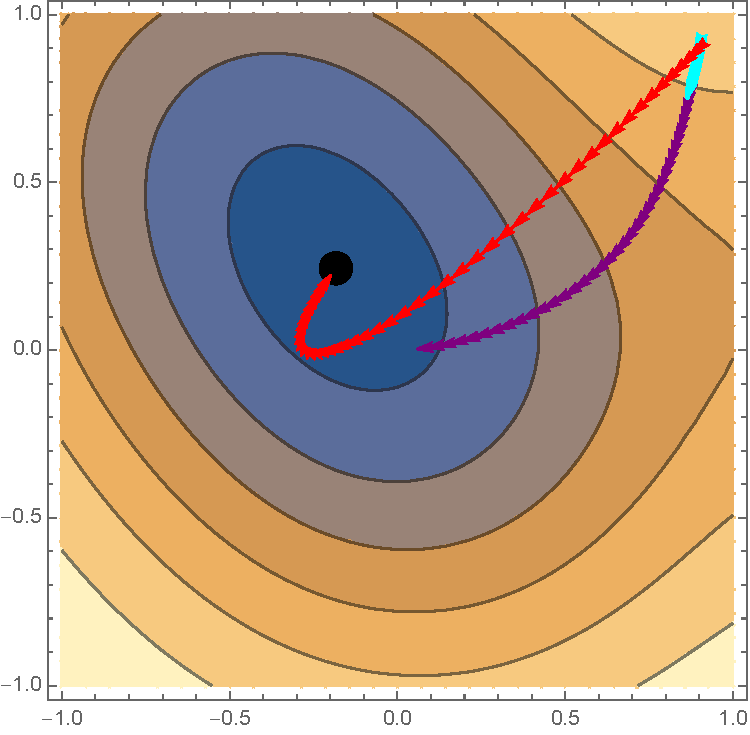
\includegraphics[width = 0.67\textwidth]{images/introduction/momentum}
	\def\c{Gradient descent routines using vanilla gradient descent (cyan), momentum (purple), and ADAM (red)}
	\caption[\c]{\c. Each routine was initialised at the same location in the top right corner of the search space and the energy function being optimised increases in value from blue to yellow. The learning rate was set to $\eta = 0.005$ and the hyper-parameters where left at their defaults $\beta_1 = 0.9, \beta_2 = 0.999$. The algorithm was ran for 100 steps and the minimum is found at the centre of the black disk. At each step the position and corresponding update step is plotted as a coloured vector. While momentum is a vast improvement on vanilla gradient descent it is outperformed by ADAM which takes a more direct line and converges more quickly. \label{fig:momemtum}} 
\end{figure}
\subsubsection{Simulated Annealing}
Simulated annealing is a heuristic non-linear optimiser that has its roots in simulating the process of a metal cooling \cite{William_H_Press2007-kb}. It works by allowing probabilistic jumps in the solution space which depend on the simulated temperature at a given time step. Suppose that $f$ is a function parametrised by $\vec{x} \in \mathbb{R}^n$ and the task is to minimise $f(\vec{x})$. An initial temperature $K$ is chosen and an annealing schedule such that for each timestep $K_t \mapsto K_0 / t$ where $\alpha \in (0, 1)$. Then, at each timestep a new parameter $\vec{x}^*$ is proposed in some appropriate neighbour set $S \subseteq \mathbb{R}^n$ which can potentially be the whole space. At each timestep the transition probability $p_t$ is calculated:
\begin{equation}
p_t = \exp\left(-\frac{f(\vec{x}^*)- f(\vec{x})}{K_t}\right).
\end{equation}
A random number $p_\alpha$ is uniformly sampled between $[0, 1]$ and if $p_\alpha < p_t$ the proposed state change is accepted. Note that any state change that results in a reduction of $f$ will be automatically accepted when $p_t > 1$. However, a change that increases $f$ may still be probabilistically accepted. While this seems counter-intuitive as an increase in $f$ moves the algorithm further away from the optimisation goal, it is useful for sampling the search space widely and allows the algorithm to more frequently break out of local minima which gradient descent algorithms may be trapped in. Finally, a trace of all available states is kept and the state that minimises $f$ is selected as the optima. 

\section{Modelling of Retinotopic Maps \label{sec:models}}
The modelling of retinotopic development has a long history with several hundreds of instances of models appearing in the literature. Models in this field are primarily data-driven and aim to explain one or mechanisms of an observed biological phenomenon. In this fashion they are tightly coupled to, and often drivers of, hypothesis driven experimental research with an observation by Goodhill reading: 
\begin{displaycquote}{Goodhill2018-ca}
Starting with Sperry’s chemospecificity hypothesis and the resulting search for molecules that might implement this, retinotectal map formation is an area where theoretical ideas have been unusually influential on experimental work. Rather than there being one ‘‘correct’’ model, competing theoretical hypotheses have all helped guide and clarify experimental results.
\end{displaycquote}
Early work in the field has been extensively reviewed by Swindale (1996), and then later by Hjorth et. al. (2015) and Gjorgjieva and Eglen (2014) \cite{Swindale1996-kk, Hjorth2015-le, Gjorgjieva2011-de}. The broad classes of mechanistic modelling alongside recent developments and several models that were not included in later reviews are now summarised. First, a comment about stability: a fundamental component of all topographic modelling. Each model is designed to either be natively static, or undergo some iterative process until it becomes so. This iterative process can be interpreted as meaningful and allow for the testing of development hypotheses, or as a convenience just allowing the final map to be generated. In either case it suggests that there is a fundamental minima to be found either as the steady state of a dynamical system, or the action of some Lagrangian (Hamiltonian). This would suggest that an energy formulation is desirable for all models, although it is not guaranteed as there is no general formulation for the inverse problem of Lagrangian mechanics. Furthermore, it is not always helpful to formulate the problem in this manner as many models are defined by computational routines which can be tricky to translate into this framework and these are sometimes best worked with directly. Nevertheless, it provides a useful abstract canvas on which to paint modelling problems. 
Some generalised approaches to modelling the three key mechanisms of competition, chemotaxis, and neural activity discussed previously will now be covered. These general techniques underpin the vast majority of models of topographic development.
\subsection{Competition}
Competition has typically been used to refer to competition for physical space or for metabolic resources and with the exception of some finely tuned chemotaxis models it forms a necessary component of every topographic model. Competition typically relates the rate of change of synaptic density at a location to the synaptic density itself. Letting $w_i(\vec{x}, t)$ represent the density of synapses at location $\vec{x}$ and time $t$ from afferent $i$ in a pool of afferents of size $N$ leads to:
\begin{equation}
\frac{dw_i (\vec{x}, t)}{dt} = f\left(\{w_j (\vec{x}, t) \}_{j=1}^N\right)
\end{equation} 
This is a general formulation but is nevertheless employed e.g. Triplett et. al. (2011) choose a highly non-linear function on both the synapses incumbent on a post-synaptic location and the number of pre-synaptic locations these synapses arrive from \cite{Triplett2011-jk}. Competition is sometimes referred to as normalisation and in these contexts it is typically simple and thought of with two dominant mechanisms: subtractive and multiplicative. Subtractive normalisation is an extreme form of normalisation given by:
\begin{equation}
\frac{dw_i(\vec{x}, t)}{dt} = Q-\alpha \sum_i w_i (\vec{x}, t),
\end{equation} 
where $\alpha$ is some constant and Q is the total weight available to some post-synaptic location \cite{Goodhill1991-fu, Goodhill1993-lk}. To stop the density from becoming negative, a physically impossible situation, one of two things are usually done: hard code a boundary at zero, or sum the total number of synapses in the system and scale it to some constant. Without some other mechanism to promote synaptic growth subtractive normalisation will lead to a rapid decay of contacts typically promoting a winner-take-all environment \cite{Miller1994-nr}. Multiplicative normalisation is given by:
\begin{equation}
\frac{dw_i(\vec{x}, t)}{dt} = -\frac{\alpha w_i(\vec{x}, t)}{g\left(\sum_j w_j(\vec{x}, t)\right)},
\end{equation}
where $\alpha$ is some constant \cite{Kohonen1982-nd, Obermayer1990-yr}. In the absence of growth this leads to an exponential decay in synaptic density between the pre-synaptic and post-synaptic locations and is therefore slower than multiplicative normalisation in the low density regime. Multiplicative normalisation therefore does not typically need a stabilisation mechanism. A natural fixed point emerges in this rule defining the density at which the growth mechanism precisely matches the decay induced by additional synapses.

To introduce competition into an energy based formulation it is sufficient to simply penalise the existence of synaptic contacts i.e. by adding energy in an energy minimisation scheme, or subtracting in a maximisation scheme. A subtractive normalisation can be modelled by associating competitive energy by summing or integrating all contacts in the system and parsing it through some function $f$:
\begin{equation}
E = f\left(\sum_i\int w_i(\vec{x}) \; d\vec{x} \right).
\end{equation}
Analogously, a multiplicative normalisation can be modelled by integrating all local contacts and parsing it through some $f$ and then summing all transformed local contributions:
\begin{equation}
E = \sum_i f\left(\int w_i(\vec{x}) \; d\vec{x}\right).
\end{equation}
\subsection{Chemotaxis \label{sec:chemotaxismodelling}}
Chemotaxis modelling has almost universally converged on two types of model: Type I and Type II  defined in Section \ref{section:chemohypothesis} \cite{Hjorth2015-le}. Both types assume that each retinal afferents affinity to a particular colliculus location is some function of the concentration of ligands and receptors at the location. In Type I systems each retinal afferent has the highest affinity for a single colliculus location but the strength of these affinity's vary. In Type II systems the receptors and ligands encoded by each afferent and each location insist on an optimal target in the colliculus for each afferent. The effect of these interactions is modelled in two general ways: an energy scheme whereby the minimal energy configuration encodes the affinity \cite{Willshaw_D_J1979-eg, Koulakov2004-ia, Tsigankov2006-uy, Tsigankov2010-on, Triplett2011-jk, Gierer1981-qc}, or a differential scheme whereby each afferent moves in accordance with a local measurement of the relevant concentrations \cite{Simpson2011-zh, Sterratt2013-ev, Gierer1983-tn, Willshaw2006-if}:
\begin{align}
E_i =& f\left(\{R^u_s(\vec{x}^u_i), L^u_s(\vec{x}^u_i): u \in \{\text{r}, \text{c}\}, s \in \{A, B\} \}\right)\\
\frac{\partial\vec{x}^\text{c}_i}{\partial_t} =& f\left(\{R^u_s(\vec{x}^u_i), L^u_s(\vec{x}^u_i) : u \in \{\text{r}, \text{c}\}, s \in \{A, B\} \}\right) 
\end{align}
where $i$ denotes the index of the afferent, $r$ and $c$ denote the retina and colliculus, and $R$ and $L$ denote the receptor and ligand concentrations of a particular subsystem respectively. In many cases the two formulations are equivalent but it is not guaranteed. In the case of multiple interacting mechanisms (Type I mechanisms require at least a competitive mechanism), the energy formulation can produce differing results to the differential mechanism depending on either the choice of energy minimisation scheme, or the initialisation location of the afferents. Simple cartoons of both differential and energy affinity maximisation schemes are shown for Type I mechanisms are shown in Figures \ref{fig:affchemotaxistype1} and \ref{fig:diffchemotaxistype1}, and Type II mechanisms are shown in Figures \ref{fig:affchemotaxistype2} and \ref{fig:diffchemotaxistype2}. 

\begin{figure}[h!]
	\centering
	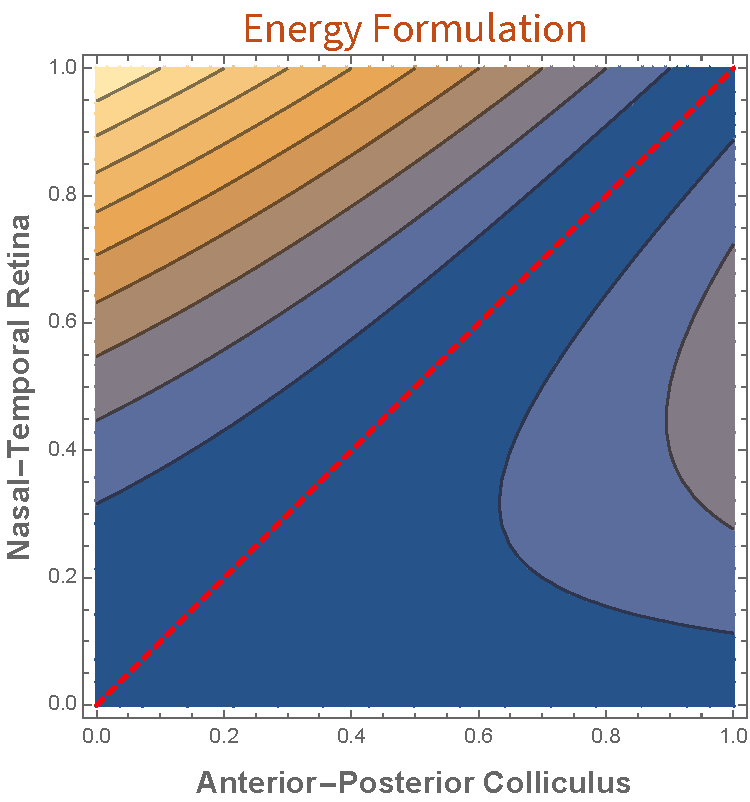
\includegraphics[width=\textwidth]{images/introduction/energy_chemotaxis_type1}
	\def\c{A simple formulation of an energy minimising scheme where the chemotactic affinity is proportional to the product of the retinal and colliculus locations along the NT and AP axes respectively.}
	\caption[\c]{\c Due to the increasing affinity along the AP axes for each retinal site there is assumed to be a competitive penalty scaling with the square of the position vector. The resulting energy profile has a non-linear shape introduced by the gradient product and mimicking the likely biological reality. The zero energy contour is highlighted in red. \label{fig:affchemotaxistype1}} 
\end{figure}

\begin{figure}[h!]
	\centering
	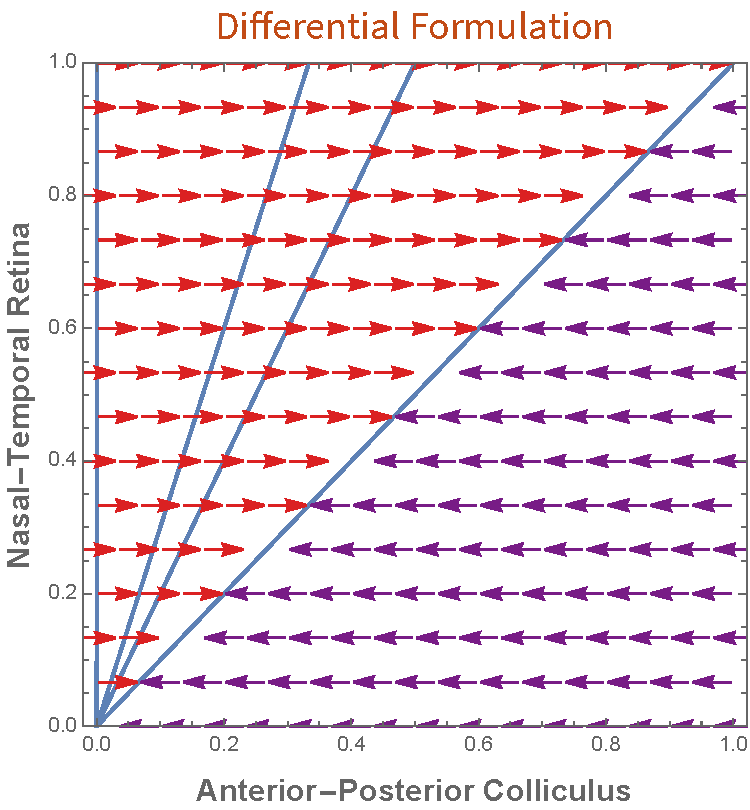
\includegraphics[width=\textwidth]{images/introduction/differential_chemotaxis_type1}
	\def\c{A simple formulation of a differential chemotaxis scheme whereby the axons in the naso-temporal retina move forward at a rate proportional to their starting location. The travelling wave front is represented by the blue fanning lines.}
	\caption[\c]{\c When first axons arrive at the hard barrier they create a barrier applying a repulsive force labelled in purple. Since this repulsive force is mediated by axonal arrival the wave front is halted along the line y=x. \label{fig:diffchemotaxistype1}} 
\end{figure}
\begin{figure}[h!]
	\centering
	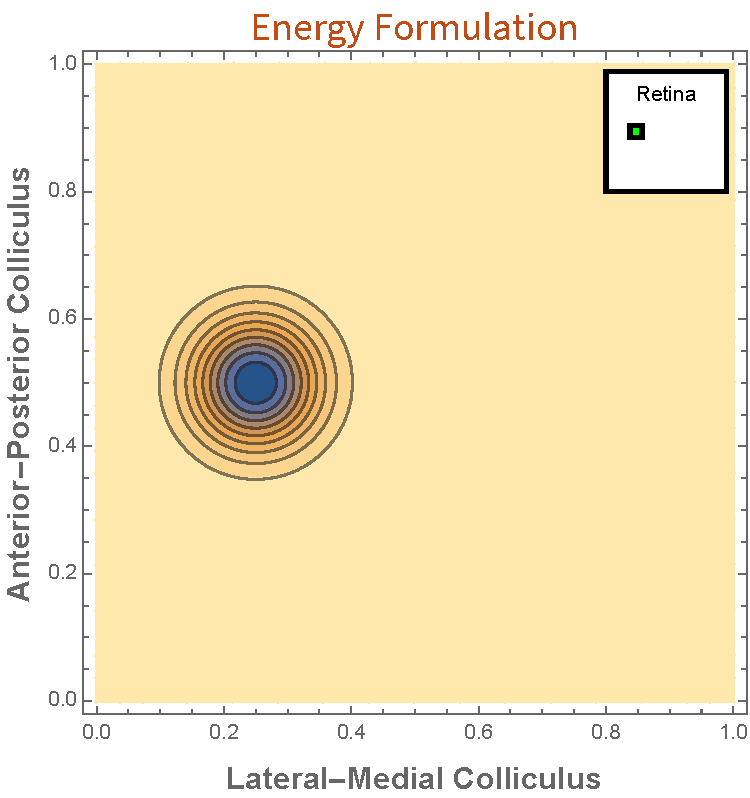
\includegraphics[width=\textwidth]{images/introduction/energy_chemotaxis_type2}
	\def\c{A simple formulation of an affinity chemotaxis scheme where the green label in the retina is given a value of both ligand and receptor. }
	\caption[\c]{\c The entire colliculus target is given a series of ligands and receptors and the quotient of products of ligands with the receptors defines the affinity. Assuming an exponential profile for all receptors and ligands $\exp(|R(\vec{x}^R)L(\vec{x}^C|)/\exp(|R(\vec{x}^C)L(\vec{x}^R)|)$; this formulation is derived from the seminal Geirer model \cite{Gierer1983-tn}.  \label{fig:affchemotaxistype2}} 
\end{figure}
\begin{figure}[h!]
	\centering
	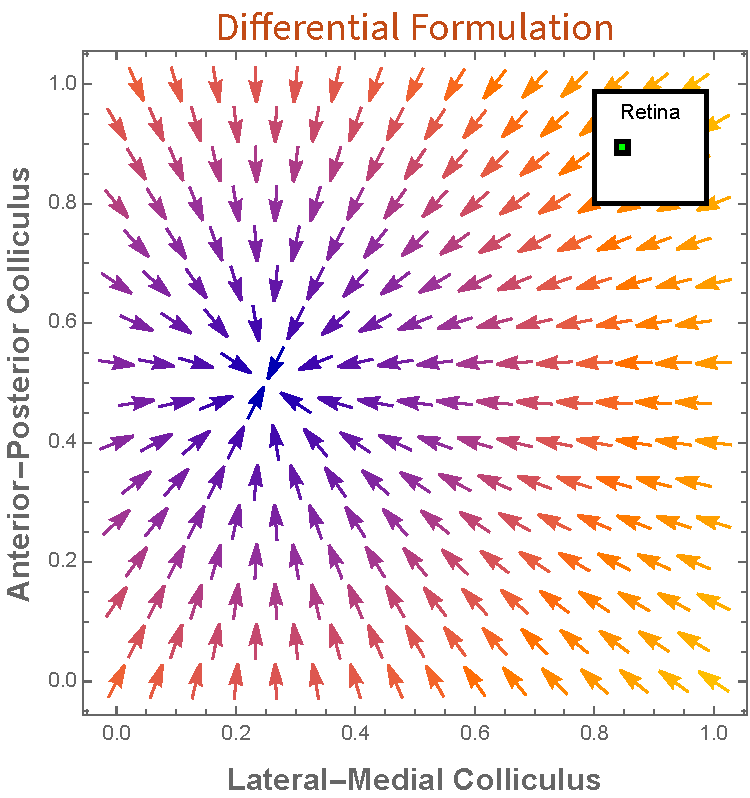
\includegraphics[width=\textwidth]{images/introduction/differential_chemotaxis_type2}
	\def\c{A simple formulation of a differential chemotaxis scheme where the green label in the retina is guided by a series of forces imposed by the interaction of the receptor and ligand values at the retinal location with various location in the target. }
	\caption[\c]{A simple formulation of a differential chemotaxis scheme where the green label in the retina is guided by a series of forces imposed by the interaction of the receptor and ligand values at the retinal location with various location in the target. The force at each location is indicated by a vector and its magnitude by a colour increasing from blue to yellow. The combinations of these forces guide the afferent into a stable location. \label{fig:diffchemotaxistype2}} 
\end{figure}

\paragraph{Fibre-Fibre Interactions}
The above cartoons deal only with fibre-target interactions with vector forces or affinities being largely composed as a result of combinations of a retinal origin position and the afferents position in the target. More complicated interactions would account for nearby afferents positions in the retina allowing for fibre-fibre chemotactic movements. This idea was the basis for the relative signalling model proposed first by Reber (2004) \cite{Reber2004-wq}. In general, models typically do not include these interactions but a more detailed discussion about them was offered by Weth et. al. (2014) \cite{Weth2014-dq}. 
\subsection{Activity \label{sec:activity}}
Chemotaxis and competition are relatively simple to describe mathematically with immediate implications. Conversely, the effects of neuronal activity on the organisation of topography is more complicated and will require detailed discussion of several mechanisms.  Neural activity is a loosely defined term which can refer to any number of collective behaviours. It is usually taken to mean a process by which a set of neurons can signal and modulate behaviour of other neurons within that set. This is most often taken to refer to spiking but several systems exhibit sub-spiking threshold activity. Furthermore, several authors take the position that rather than individual spikes being the relevant quantity it is the spiking rate which encodes relevant information.
\paragraph{Neuronal Spiking}
There are three major classes of model for describing spiking behaviour: biophysical, integrate-and-fire, and Poisson. The biophysical model is typically inspired by the work of Hodgkin and Huxley and is concerned with the non-linear modelling of membrane voltage along a cell body with three response variables \cite{Hodgkin1952-yi}. The Hodgkin-Huxley model has been extensively developed and computational packages such as neuron can model individual compartments of a neuron and its firing in detail \cite{Carnevale2006-gn}. In general, these models are too computationally intensive to apply to large scale studies and will not be detailed further.

A simpler model that captures much of the underlying biophysics is the integrate-and-fire which is desirable for its computational-efficiency to accuracy trade-off \cite{Abbott1999-ms, Burkitt2006-ne}. This class of model typically assumes a membrane potential variable $v_i(t)$ and a response variable $u_i(t)$ and some input $I_i(t)$ at a node $i$, along with a set of threshold parameters $\vec{P}$ which specify the threshold potential at which a spike occurs and what the potential and response variables should be reset to after this spiking event. These models have the general form:
\begin{align}
&\dot{v}_i(t) = f(u, v, I; \vec{P})\\
&\dot{u}_i(t) = g(u, v, I; \vec{P}),
\end{align}
for some general functions $f$ and $g$. The functions can be relatively simple as in the leaky integrate-and-fire neuron where $f(v, I) = \alpha - v + I$ for some constant $\alpha$ and $g = 0$. They can also be relatively complex aiming to capture almost all of the underlying bio-physics while maintaining efficiency; see Izhekvich for a detailed formulation \cite{Izhikevich2003-ht}. 

The simplest model in terms of computational efficiency of spike generation is the Poisson model. In this model a neuron is assumed to have a possibly time-varying firing rate $r(t)$ and for a given time interval $dt$ is assumed to release $r(t) dt$ spikes. The probability of releasing a spike is independent of any spikes that have occurred previously and thus the probability distribution is Poisson. Therefore, a time-series of activity can be generated by partitioning the time into sufficiently many intervals of length $dt$ and for each interval comparing a random number sampled from a uniform distribution with $r(t)dt$: if the random number exceeds $r(t)dt$ then there is no spike and vice-versa. This spiking model, while cheap and relying on simplifying assumptions, has been shown to capture many properties of the underlying neural activity distributions \cite{Burkitt2006-wq, Burkitt2006-ne}.

\paragraph{Neuronal Networks}
A natural extension from these spiking models of neurons is to model portions of the brain as a network of coupled nodes that each exhibit these spiking dynamics. A network in network science is an ordered triple $\mathcal{R}(N,E,f)$ where $N$ is a set of nodes in the network, $E$ is a set of edges and $f$ is a mapping from an edge in $E$ to a pair of nodes in $N$ \cite{Barabasi2016-wx}. 

Networks can be directed or undirected. In a directed network the edges can have a specific direction attached to them so for each pair of nodes $i$ and $j$ there are two possible edges; $f: E \rightarrow N\times N$. Networks can also be weighted or unweighted. In a weighted network a real number is assigned to each edge by a weight function $w: E \rightarrow \mathbb{R}$. All of this information can be contained in a matrix called the adjacency matrix $\mathcal{A}$. The entries of the adjacency matrix $\mathcal{A}_{i,j}$ are given by the weight function of the edge between nodes $i$ and $j$ and are zero if no edge exists between them.

Each node on the network may exhibit some dynamics. Consider a set of parameters $\vec{v}_i$ which describe the dynamics of a node $i$. The dynamics of each node will be dependent on some internal dynamics as well as some input from other nodes which connect to it. If there are $n$ such nodes in the system this can be summarised as:
\begin{equation}
\dot{\vec{v}}_i=F(\vec{v}_i)+\sum_{j=1}^{n} G(\mathcal{A}_{i,j},\vec{v}_i,\vec{v}_j,\dot{\vec{v}}_j).
\end{equation}
The function $F$ determines the effect of the internal dynamics and the function $G$ determines the input of the $j$-th node to the dynamics as a function of the weight of the edge between them, the dynamics of the $j$-th node and the state of the $i$-th node. Solving this equation will completely determine the dynamics of the system. In general there may be no analytical solution to this equation.

A neural network may then be constructed by associating each node with a neuron and each edge with a synaptic connection. For a simple consideration, consider a leaky-integrator model where activity on the $i$-th neuron is given by $u_i$, the time scale of the leak is given by $\tau$, the activation function is given by $f$ and the $j$-th neuron is coupled to the $i$-th with a synaptic weight $w_{ij}$. It is assumed here that a spike in the $j$-th neuron induces a rapid change in the potential of $u_i$ of $w_{ij}$ by the release of neurotransmitters and then this change decays exponentially; a simplistic form of synaptic processing. The network dynamics are then given by:
\begin{equation}
\tau\dot{u}_i(t)=-u_i(t)+\sum_{j=1}^{n}w_{ij}f(u_j(t)).
\end{equation}
In this formulation the weighting matrix $w_{ij}$ informs both the existence of a synaptic connection and its type, inhibitory or excitatory (negative and positive weights respectively). This network is undirected as many neurons only feed-forward to other neurons. The effect of an input stimulus can be examined by artificially injecting current into a node, or subset or nodes, and examining the effect on the dynamics of the network.

\paragraph{Neural Field Theories}
The large number of synapses and neurons and the observation that neurons behave in a similar fashion to each other leads itself to the idea of a continuum model based on some averaging process. The activity of a location of neurons $u(\vec{x},t)$ is assumed to obey the same synaptic processing dynamics and have a change in potential due to the activation (spiking) of other connected populations. These models therefore typically involve a partial integro-differential equation with a linear operator dictating local temporal evolution and spatial convolution, possibly with delay, integrating responses from other locations.

The seminal model by Wilson and Cowan (1973) assumed that each location had excitatory and inhibitory populations which had some refractory response \cite{wilsoncowan2}. These populations were coupled to each other and themselves with the kernels $W_{EE}$, $W_{EI}$, $W_{IE}$ and $W_{II}$. They then obeyed the pair of coupled partial integro-differential equations \cite{wilsoncowan1, wilsoncowan2}:
\begin{align}
\frac{d E(\vec{x},t)}{dt} = & -E(\vec{x},t) + (1- r_E E(\vec{x},t)) S_E \left[ \int_{\Omega} d\vec{y} W_{EE}(\vec{x},\vec{y}) E(\vec{y},t)- W_{EI}(\vec{x},\vec{y}) I(\vec{y},t) \right]\\
\frac{d I(\vec{x},t)}{dt} = & -I(\vec{x},t) + (1- r_I I(\vec{x},t)) S_I \left[ \int_{\Omega} d\vec{y} W_{IE}(\vec{x},\vec{y}) E(\vec{y},t)- W_{II}(\vec{x},\vec{y}) I(\vec{y},t) \right],
\end{align}
where $S_E$ and $S_I$ represent the expected proportion of neurons in either the excitatory or inhibitory populations that receive at least the threshold excitation per unit time and $r_j$ represents the refractory periods for excitatory and inhibitory populations for $j=E$ and $j=I$ respectively. The advantage of this model is flexibility. It allows one to specify completely the spatial interactions between different excitatory and inhibitory populations, the non-linear response to activation of different spatial regions and the refractory period for these populations.

By making some assumptions about the connectivity and nature of populations of neurons Amari (1977) simplified this model writing it in terms of the average membrane potential $u(\vec{x},t)$ \cite{Amari1977-gc}. Presume that there $m$ different layers of neurons with each layer possessing neurons only of the same type, then the activity in a location of the $i$-th layer will be determined by internal dynamics of that neuron type and input from the other layers:
\begin{equation} \label{ch2Amari1}
\tau_i \frac{du_i(\vec{x},t)}{dt} = - u_i(\vec{x},t) + \sum_{j=1}^{m} \int_{\Omega} d\vec{y} W_{ij}(\vec{x},\vec{y}) f_j(u_j(\vec{y},t-d_{ij}(\vec{x},\vec{y}))) + h_i + s_i(\vec{x},t),
\end{equation}
where $W_{ij}$ is represents the connectivity kernel between layers, $d_{ij}(\vec{x},\vec{y})$ represents the delay between the $\vec{x}$ location in the $i$-th layer and $\vec{y}$ location in the $j$-th layer, $s_i(\vec{x},t)$ represents the deviation from average stimulus being presented at $(\vec{x},t)$ and $h_i$ represents the deviation of average stimulus from some resting threshold $r_i$. 

Now consider that there are only inhibitory and excitatory populations in a single layer i.e. encapsulate all the neuron types into a single structure. Assume that the average membrane potential $u$ at some location is the combination of the activity levels of inhibitory and excitatory populations. Also assume that they both fire at a rate determined by the average potential, $f(u)$, and evolve on the same time scale. Kernels that specify excitatory-excitatory, excitatory-inhibitory, inhibitory-excitatory and inhibitory-inhibitory synaptic connections can be replaced with two kernels: $W_I(\vec{x},\vec{y})$ and $W_E(\vec{x},\vec{y})$. These kernels specify the input into the inhibitory and excitatory populations at location $\vec{x}$ given an average activation level, or firing rate, $f(u)$ from location $\vec{y}$. Since average population response is considered to be the combination of the inhibitory and excitatory response and they evolve with the same time scale they are written in terms of a single signed kernel $W$:
\begin{equation} \label{ch2Amari2}
\tau \frac{du(\vec{x},t)}{dt} = - u(\vec{x},t) + \int_{\Omega} d\vec{y} W(\vec{x},\vec{y}) f(u(\vec{y},t)) + h_i + s(\vec{x},t),
\end{equation}
where $W(\vec{x},\vec{y})= W_E(\vec{x},\vec{y})-W_I(\vec{x},\vec{y})$ is that signed kernel. If the inhibitory connections from $\vec{y}$ to $\vec{x}$ dominate then the activation of location $\vec{y}$ will have an inhibitory effect on $\vec{x}$ and vice versa. This formulation can still incorporate delays if they are same for both inhibitory and excitatory populations. It is useful because it incorporates both inhibition and excitation into the sign of the kernel, despite inhibitory and excitatory neurons and synapses being different biological structures.

The Amari equation can also be seen as the continuum average of the neural network with leaky integrator dynamics, where the connectivity matrix $w_{ij}$ is replaced with the connectivity kernel $W(\vec{x},\vec{y})$ and the summation is replaced with an integral.
\subsection{Neuroplasticity}
Neuroplasticity is the process by which neurons change their synapses. It is thought to be mediated by correlated pre-synaptic and post-synaptic activity. In Chapter \ref{chapter:biology} Hebbian learning, and in particular STDP, was discussed as a description for how these synaptic dynamics may be governed. This section will detail several mathematical implementations of Hebbian learning, in particular STDP, and describe how STDP may be implemented in a field theory, which concerns itself primarily with firing rates and not with individual spiking events.
\paragraph{Hebbian Learning}
There are many challenges with implementing a Hebbian learning rule based simply on the notion of correlated pre-synaptic and post-synaptic firing rates. Let the pre-synaptic firing rate in the $i$-th neuron be represented as $p_i(t)$ and the post-synaptic firing rate in the $j$-th neuron as $u_j(t)$ respectively, and let the synaptic weight be represented as $w_{ij}$. One such notion is to simply calculate the product of the deviations from the average firing rates $\bar{p}$ and $\bar{u}$:
\begin{equation}
\dot{w}_{ij}(t) = w_1(p_i(t)-\bar{p})(u_j(t)-\bar{u}),
\end{equation}
where $w_1$ is a scaling constant. The issue here is that the process results in a feedback loop, initially positively correlated signals receive a synaptic boost, in turn making them more likely to be correlated upon further stimulation and vice versa for initially negatively correlated signals. This means that all firing rates tend to decay, or grow without bound. It is therefore necessary to somehow stabilise this process. A simple method is to impose saturation limits on the weights: a synaptic weight may grow to $w_{\text{max}}$ or decay to $w_{\text{min}}$. To stabilise the firing rates some competitive decay term, which may depend on the post-synaptic firing rate,  must be added:
\begin{equation}
\dot{w}_{ij}(t) = w_0(t,w_{ij},u) + w_1(p_i(t)-\bar{p})(u_j(t)-\bar{u}).
\end{equation}
This term affects all synapses, although it may be weighted by the current synaptic strength, making it a global adjustment. If this decay term is constant the adjustment is referred to as subtractive, and if the decay term is dependent proportional to the synapses current strength it is referred to as multiplicative. In general, multiplicative adjustments are less competitive than their subtractive counterparts \cite{Abbott2000-gl}.
\paragraph{Spike Timing Dependent Plasticity \label{sec:nftplsaticity}}
Spike timing dependent plasticity (SDTP) is a form of Hebbian learning in which the dynamics of synaptic change are governed by relative timing between a pre and post-synaptic spike \cite{Abbott2000-gl}. It has been experimentally observed on the synaptic level, making it useful for mathematical model creation and subsequent analysis, but the precise physiological mechanisms remain unknown \cite{Froemke2002-be, Zhang2000-lb}. There are several different functional forms of STDP, most of which possess some structure around the origin; typically they are anti-symmetric or symmetric. The synaptic change caused by a pair of pre and post-synaptic spikes is assumed to be independent between pairs. Therefore, the total synaptic change in a given time window is found by computing the synaptic change induced by each pair, individually, and then summing the changes over all pairs.

This work shall focus on two representative forms of STDP, one that is symmetric around the temporal origin, and one that is anti-symmetric \cite{Abbott2000-gl}. Henceforth, correlation dependent plasticity (CDP) will refer to plasticity that is symmetric around the temporal origin and STDP to plasticity that is anti-symmetric. Other forms of plasticity shall not be considered. CDP rewards signals that are closely correlated in time STDP rewards casually correlated signals. A canonical form of these two learning rules is defined then by a plasticity window $H$:
\begin{equation}
H(\tau) = \begin{cases} \label{STDPcanonicalform}
A_+ \exp(-\frac{\tau}{t_p}) &\qquad \tau >0\\
A_- \exp(\frac{\tau}{t_p}) &\qquad \tau <0 
\end{cases}
\end{equation}
CDP is found by setting $A_+=A_->0$ while STDP is found by setting $A_+=-A_->0$ \cite{Robinson2011-ve, Abbott2000-gl}. Here the time-scale over which plasticity occurs, $t_p$ is the same for both positive and negative temporal separation. The synaptic change is computed by sliding the plasticity window over each post-synaptic spike and summing the changes induced by the correlation with each pre-synaptic spike. The Fourier transforms of these learning rules are given by:
\begin{align}
& \hat{H}_{CDP} (\omega)= \frac{2A_+}{1+\omega^2 t_p^2} \label{CDPrule} \\ 
& \hat{H}_{STDP} (\omega)= \frac{2A_+ i \omega t_p }{1+\omega^2 t_p^2}. \label{STDPrule}
\end{align}
\paragraph{Neuroplasticity in a Field Theory}
The plasticity window is defined for pairings of single spikes on a given neuron. Robinson (2011) \cite{Robinson2011-ve} showed that it is possible to derive a mean synaptic change averaged over many neurons in two neuronal populations by considering the post-synaptic spike rate $U$ and the incoming spike train $A$. To do this an average is taken over some moving window of width $T$ which is chosen to be longer than the time scale of the plasticity window and of the inverse frequencies of $U$ and $A$, but shorter than that of the long term plasticity changes. The average change in plasticity, S, is then expressed as:
\begin{equation}
\frac{dS(\vec{x},\vec{y},t)}{dt} = S_0 \int_{-\infty}^{\infty} \langle U(\vec{x},t+\tau) H(\tau) A(\vec{y},t) \rangle d\tau,
\end{equation}
where $S_0$ is some scaling factor. It is then argued that large scale behaviour is governed by a steady state and temporal perturbations to this state; writing the pre-synaptic and post-synaptic expressions as perturbations from steady states, $U(\vec{x},t) =U^{(0)} + \delta U(\vec{x},t)$ and $A(\vec{x}^\prime,t) =A^{(0)} + \delta  A(\vec{x},t)$ respectively. These are then Fourier transformed and the average value is evaluated by the zero-frequency component. It is noted that the zero-th order terms give no net contribution, and the terms linear in the perturbations give no net contribution because the perturbations average to zero. Fourier transforming and evaluating at the zero-th frequency yields:
\begin{equation} \label{robinsonSTDP}
\frac{dS(\vec{x},\vec{x}^\prime,t)}{dt} = \frac{S_0}{2\pi} \int_{-\infty}^{\infty} \delta \hat{U}(\vec{x},\omega) H(\omega)^* \delta\hat{A}(\vec{x}^\prime,\omega)^*d\omega.
\end{equation}
Where $\delta\hat{A}$ and $\delta \hat{U}$ are the Fourier transforms of the pre-synaptic and post-synaptic perturbations respectively and the star denotes conjugation. This expression is useful because it allows one to to express the changes in synaptic coupling between two neuronal populations by examining linear temporal perturbations from the steady state in the pre-synaptic and post-synaptic firing rates. It is simply necessary to adopt an appropriate neural field theory to compute these perturbations. It also allows mathematical analysis of systems level plasticity on a more biologically solid foundation with the STDP rule being more biologically accurate than the typical Hebbian implementations.
\subsection{Activity Based Topographic Development}
The seminal models for activity based topographic development were integrate-and-fire network based simulations first examined by Willshaw and van der Malsburg \cite{Willshaw1976-ew}, and a field theory based model proposed by Amari \cite{Amari1977-gc}. They both employ the Hebb rule and a multiplicative normalisation competitive mechanism.

Amari's theory of topographic development was first developed in 1-dimension with periodic boundary conditions and a simple Hebbian mechanism and two key assumptions: a Heaviside firing rate, and a Hebbian rule which was computed on a time-scale that allowed a constant stimulus in the retina to tend equilibrium in the SC \cite{Takeuchi1979-zy}. This work was extended by Zhang (1990) to relax the assumption of the firing function to be a more realistic sigmoid function and by Taylor (1999) to be realised in a 2-dimensional setting \cite{Zhang1990-ve, Taylor1999-mv}. The Detokaris-Rougier model was developed for somatosensory topographic systems but in the abstract translates to retinotopic mapping in a 2D setting. The authors were able to demonstrate the reorganisation of the topographic map represented by a field after repeated stimulation and application of a Hebbian mechanism \cite{Detorakis2012-eh}.

\paragraph{Distance Dependent Correlation \label{sec:distancecorellation} }
More recently, the field has converged on the notion of distance-dependent correlations to model activity based mechanisms in development \cite{Grimbert2012-cd, Triplett2011-jk}. This assumption has been largely driven by the study of spontaneous retinal waves which demonstrate an exponential decay in measures of correlation in these patterns of neural activity with an analogous set of waves measured in the colliculus \cite{Stafford2009, Ackman2012-uu}. These models essentially assert that each retinal location has the ability to potentiate colliculus neurons proportional to the connection strength with that retinal location. If two sites are co-active then they will potentiate the colliculus defining a set of active synaptic pairs. The assumption is that each of these pairs when coupled have an affinity that is proportional to the product of the correlation between them. The affinity for a pair of synapses $i$ and $j$ is then:
\begin{equation}
E_{ij} = C_R\left(\lVert \vec{x}^R_i - \vec{x}^R_j \rVert_2\right)C_C\left(\lVert \vec{x}^C_i - \vec{x}^C_j \rVert_2\right),
\end{equation}
where $\vec{x}_k^R, \vec{x}_k^c, C^R, C^c$ denote the positions and correlations in the retina and colliculus respectively and $\lVert \cdot \rVert$ is the Euclidean 2-norm. The correlation function is usually taken to be an exponential or a Gaussian function. The solution is found by maximisation of this affinity over all possible synapse pairs. This process in general is highly non-linear and unlike affinities with chemotaxis the structure of local maxima is not immediately provable. The efficacy as a mechanism for topographic mapping can, however, be deduced. Fix all synapses associated with a single neuron $i$ and consider maximising the affinity by placing $N$ new synapses conditional on this neurons location. It is apparent that distal neurons in the retina suffer immediate penalty and will not be useful in maximising the affinity. Furthermore, synapses that are close in the retina but distal in the colliculus suffer the same penalty. The optimal solution for a fixed number of synapses is then to place them all as close as possible creating a local topographic domain. The complexity comes from the highly symmetric nature of the correlation function: a domain can be translated and rotated freely when subject to no other constraints. The removal of global guidance from chemotaxis means that highly ordered domains will occur which are topographic in their interior but discontinuous along a finite number of boundaries thereby satisfying the constraint for a local minima. This behaviour is shown in Figure \ref{fig:activitydomain}.

\begin{figure}[h!]
	\centering
	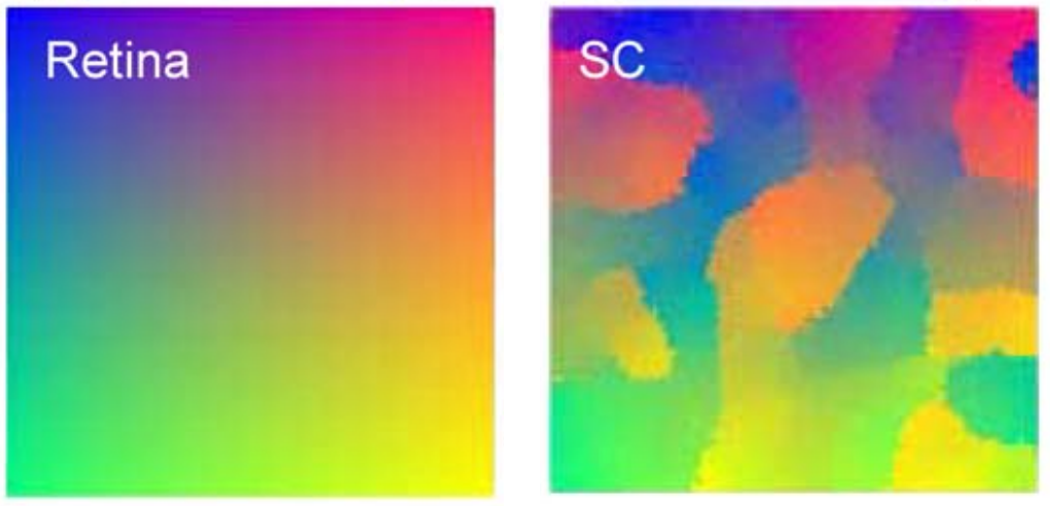
\includegraphics[width = \textwidth]{images/introduction/koulakov_domains}
	\def\c{When the affinity is no longer constrained in a global fashion by chemical guidance cues neuronal activity drives the formation of independent topographic domains. }
	\caption[\c]{\c Each domain is topographic up until its boundary where it permits a discontinuity. These discontinuities imply that the system has not found a global minima, but they also represent local energy minima indicating they are stable. Figure adapted from Tsigankov and Koulakov (2006) \cite{Tsigankov2006-uy}\label{fig:activitydomain}} 
\end{figure}

In the differential formulations these considerations mean that co-activation of retinal neurons $i$ and $j$ result in the synapses defining their arbours moving towards the conjoined centre of mass. This results in a refinement of synaptic arbours to be as geometrically close as possible to synaptic arbours with which their retinal cells receive the most co-activation. The movement is stronger when the retinal origins are also closer to each other: distance-dependent correlation leads to the desired phenomenological effect. This is shown in Figure \ref{fig:activityattraction}.
\begin{figure}[h!]
	\centering
	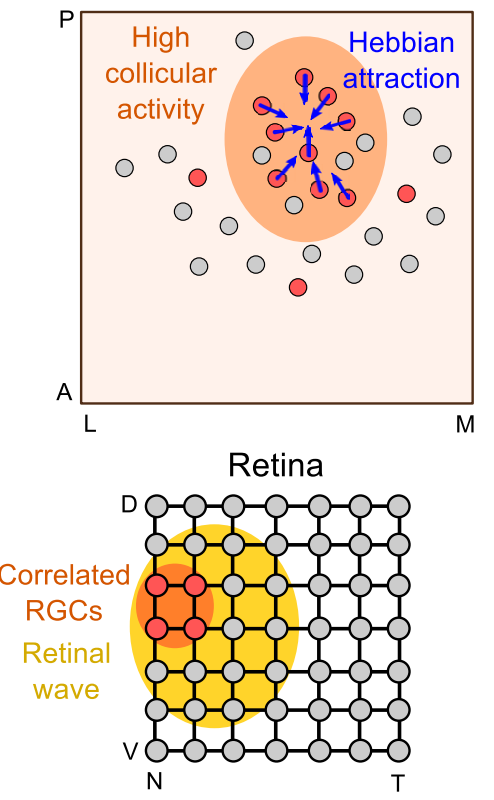
\includegraphics[width = 0.67\textwidth]{images/introduction/cang_attraction}
	\def\c{The effect of co-activation of neurons in the retina is to move their synaptic presence closer to their shared centre of mass. }
	\caption[\c]{\c This effect is most pronounced when retinal cells are frequently co-active. A distance-dependent correlation function then insists on shared topographic domains for neighbouring retinal cells due to a pronounced mutual co-activation of nearby retinal cells. Figure adapted from Grimbert and Cang (2012) \cite{Grimbert2012-cd} \label{fig:activityattraction}} 
\end{figure}


\subsection{Mechanical-sensing Models}
Mechanical sensing is proving to play an important role in the development of the retinotopic projection. Despite this there have been no models dedicated to  explaining and predicting the effects of this mechanism. The role of mechanical sensing with respect to topographic mapping has been most intensively studied in the Xenopus model system and has been used to explain the characteristic turn made by the axonal bundle originating in the retina en route to the tectum \cite{Koser2016-tm}.

\subsection{Unified Models}
More recently the field has converged on unified models involving multiple mechanisms and usually to explain a particular dataset. These models typically apply the general principles outlined above. Four key recent models are detailed which highlight the differences and similarities in the above approaches and demonstrate what steps the field needs to take next.

\subsubsection{Godfrey-Swindale-Eglen}
The Godfrey-Swindale-Eglen (GSE) model is a highly detailed model that aims to be as biophysically accurate as possible with detailed mechanisms included for several known biological processes: axon growth and branching via molecular guidance cues, synapse generation and deletion mediated by trophic factors, a conductance based integrate and fire model of neuronal activity, homeostatic mechanisms for balancing neuronal firing rates, and STDP \cite{Godfrey2009-ts}. There are several potential implications of perturbations to each individual mechanism which will not be elaborated. 
\paragraph{Mechanisms}
The axonal growth model assumes that an axon is composed of a series of individual segments and at each time step there is the possibility of an axon segment growing, or branching. At each segment of each axon there is an affinity associated with a chemotactic cue and a trophic factor and is modelled as a differential equation. The chemotactic affinity for a branch was given by a lock-and-key mechanism which had different functional forms but amount to the same preference for a single location in the target. The different forms mediate the branching process to help the model reproduce the interstitial branching effect \cite{McLaughlin2003-nf, McLaughlin2003-co, Hindges2002-rt}. The growth and branching processes are mediated by an axonal resource which is governed by a differential equation coupled to affinity.

Every five seconds there is a probability of an axon growing or branching which functions of the resources available to the segment and the threshold for each of these. The thresholds are fine tuned arbitrarily, as with the chemo-affinity, to control the phenomenological aspect of branching observed experimentally. Any growth segment with no children also has the possibility of contracting calculated as a function of resources and some unique threshold. The vector along which a growth occurs is a mix of the vector of its parents orientation and the orthogonal vector to the orientation. The relative proportions are controlled so that branching is largely orthogonal with a perpendicular offset  and growth is largely perpendicular with an orthogonal offset. The relative amount of offset is tuned by some parameter. Probabilistically it is relatively clear to see that with a lock-and-key affinity profile and some method by which to maximise this profile each axon will find its correct target. What is novel in this approach is that it allows for the full developmental time-course to be explicitly modelled but requires a high degree of tuning. 

In addition to the growth of an axon the model allows for the generation and deletion of individual synapses. This process is established after the initial growth stage is complete and the neuronal activity mediated through retinal waves stage is initiated. During this stage the axons are still allowed to grow. A standard integrate-and-fire model was employed with a variable conductance mediated by a sigmoid of the ratio between the current firing rate and the target rate to model the post-synaptic firing events. The excitation input to a neuron was modelled as the sum of all incoming synaptic weights scaled to a homeostatic rate function. Pre-synaptic firing events were generated using a Poisson process that was activated when a certain level of recorded calcium activity was exceeded. Synaptic weights were finally scaled according to pre-synaptic and post-synaptic time correlations using an STDP rule. This stage was allowed to continue for 60 hours.
\paragraph{Findings}
The authors examined two major scientific questions: the developmental time course of the map, and the $\beta2^{-/-}$ knock-out. They found that with sufficient tuning the model was able to accurately reproduce several features of the wild-type phenotype notably interstitial branching and a pattern of establishing a coarse topographic map followed by a refinement period. Notably, the model suggests that molecular guidance has a limiting effect on refinement which is a point corroborated by a theoretical analysis from Goodhill \cite{Goodhill2016-ck}. Furthermore, when the activity based refinement period was activated prematurely the authors observed a near complete disruption of the map supporting the notion of a critical period and experimental evidence for the relative timings of guidance and refinement. 

The authors further suggest that a mechanism for synapse creation and deletion mediated by derived trophic factors is sufficient for refinement and that a STDP mechanism contributes little to no effect in the processing of map formation. This prediction was made by completely disabling the STDP mechanism and allowing the map to develop whereby the plasticity is mediated by the number of synapses on a target rather than their strength. However, the reverse experiment was not performed with trophic based synapse creation being restricted and STDP driving synaptic reorganisation. Therefore, the model allows for the possibility of STDP also being sufficient for map formation.

The authors also studied the $\beta2^{-/-}$ knock-out by approximating the data presented by \cite{Stafford2009, McLaughlin2003-nf}. The retinal cells were assumed to be in a bursting state when recorded calcium levels exceeded a threshold allowing the rate of the Poisson process generating spikes in the model to be up-regulated. In this way several activity patterns were examined and the model was able to accurately predict the phenomenology of the $\beta2^{-/-}$ mutant: larger projective and receptive fields. Notably, the authors acknowledge that the quantitative prediction was an order of magnitude different to the observed measurement but this could likely be due to the activity properties of the $\beta2^{-/-}$ not being fully understood. The authors further conjecture that the it is not the particular properties of the waves themselves but the correlation patterns that the waves establish between individual neurons that principally explain the data; see Section \ref{sec:activity}. This is supported by an experiment where activity is entirely decorrelated yielding a lack of retinotopic refinement \cite{McLaughlin2003-yy}.
\paragraph{Key Issues}
The model is able to accurately reproduce several aspects of regular wild-type development in addition to qualitatively reproducing the $\beta2^{-/-}$ knock-out. However no other mutants were described. The lock-and-key mechanism used for chemotaxis means that most chemotactic perturbations will likely be qualitatively accounted for, however examination of the $Math5^{-/-}$ mutant would be of keen interest given the resource not space based competition mechanism.

Each stage of the model has required a degree of parameter tuning completed by the expert. To rigorously establish these parameters scientifically it would be valuable to estimate these tuned parameters statistically with reference to a dataset. However, the computationally demanding runtime makes this prohibitively expensive. The model is therefore most useful as a detailed phenomenological explanatory tool.  A large degree of the runtime arises from the sheer complexity of the model. It involves simultaneous solutions of coupled differential equations corresponding to several mechanisms coupled on thousands of indexes. The authors acknowledge that: ``The complexity of the model made it a practical impossibility to pre-define numerical quantities for the large range of mechanisms represented". Given the number of degrees of freedom it is reasonable to assume that almost any data can be explained with sufficient parameter tuning. While this can offer biological insights it presents a challenge to model interpretability and confidence.

The GSE model while incredibly detailed has several key shortfalls: time, complexity, and to quantitative inaccuracy. The model takes approximately five days to converge which makes exploratory analysis without access to unreasonable amount of computation power impossible. Therefore, the model can, if accurate, only be used for confirmation studies. The computational intensity also limits the models statistical capabilities and makes Bayesian fitting almost impossible. The complexity also allows for a level of fine tuning . Finally, the only phenotype ($\beta2^{-/-}$ mutant) that the model was tested against was quantitatively inaccurate when compared to data.
\subsubsection{Grimbert-Cang}
The Grimbert-Cang model uses two-stage development process which is designed to mimic the development process \textit{in vivo}: retinal afferents are placed in the colliculus stochastically according to their receptor ligand profile using stochastic sampling, then a differential equation formulation of competition and activity is used to evolve the afferents location to their final position. 
\paragraph{Mechanisms}
For the A system stochastic sampling proceeds by defining a probability distribution proportional to a combination of receptors and ligands in both the afferents retinal location and the potential location in the colliculus. This probability is composed as a product of a forward probability (forward signalling) and reverse probability (reverse signalling):
\begin{equation}
P(x_R, x_C) = P_F(x_R, x_C)P_R(x_R, x_C),
\end{equation}
where $P_F$ and $P_R$ are both sigmoid functions of the relative difference in ligand and receptor in the retina and colliculus. Since the two combinations (retinal-receptor to colliculus-ligand, and colliculus-receptor to retinal-ligand) are counter-graded with each other the sigmoid defined by $P_R$ and $P_F$ will have different parity implying a unique location where the probability is maximised. For each axon at $x_R$ a branch location $x_C$ is chosen with uniform sampling and retained with probability $P(x_R, x_C)$. The B system is computed in a simpler fashion each retinal axon is associated with a perfect position $y$ and sampled with an error $E$, then an additional error $e_i$ is added for each branch. This procedure therefore generates a probabilistic arbor for each axon. Since the placement function has unique maximal probabilities this model is a Type II mechanism. Once all branches have been placed the algorithm proceeds with solving the differential equation:
\begin{equation}
\frac{d \vec{x}^C_i}{dt} = \alpha \sum_j W(\vec{x}^R_i - \vec{x}^R_j) F(\vec{x}^C_i - \vec{x}^C_j) - \beta \nabla_CD(\vec{x}^C_i),
\end{equation}
where $\vec{x}^Z_i$ denotes the retinal $Z = R$ and colliculus $Z = C$ locations of the $i$'th axon, $W$ is a function that is assumed to contain all information about the correlation effects of retinal waves and there implicit effect on axonal arborisation, $F$ contains similar information but instead models a ``Hebbian attraction", and $D(\vec{x})$ represents the sum over all axons of a series of Gaussian's centred around the branches locations. The effect of the second term is immediate as in isolation it models the diffusion equation. Thus, it encourages the axonal centres to move down the concentration gradient and with boundary conditions that prevent loss of material will result in the branches being uniformly distributed throughout the target. The first term implicitly adopts the argument laid out in Section \ref{sec:distancecorellation} with a Gaussian correlation in the retina and a non-linear function in the colliculus given by $F(\vec{x}) = K(1-\lVert\vec{x}\rVert_2^2/\theta^2)\vec{x}$ for some $K$, $\theta$ and restricted to the semi-positive domain by mapping all negative values to zero.
\paragraph{Findings}
Using the model the authors examined several phenotypes: WT, the EphrinA triple knock-out, the EphA3 heterozygous and homozygous knock-ins, the EphA7 knock-out, and the p75Ntr knock-out. The model was able to accurately reproduce the phenomenology of each of these phenotypes which in the case of the receptor-ligand perturbations is expected as the model is constructed as a Type II lock-and-key mechanism for chemotaxis. The p75Ntr knock-out involves disrupting a receptor-ligand reaction but is less well understood with experimental results suggesting it is critical for reverse signalling to occur \cite{Lim2008-bq}. The authors found they were able to broadly recreate the phenomenology of the mutant by disabling reverse signalling and tweaking the role of competition which they suggest implicates p75Ntr in retinocollicular competition.
\paragraph{Key Issues}
The authors examined the effect of removing competition on the final maps in some sense in their exploration of the p75Ntr knock-out. They first demonstrate that decreasing the strength competition decreases the total area covered by arbors in the colliculus. It is not clear here if they define the total area to be the union of sets defined by the area function of each retinal axon branch, or conversely the area of the union of all branches. This is a subtle difference with important implications for the $Math5^{-/-}$ mutant. In the second case, provided the map was oriented at the correct boundary, the model would predict the effect of the mutant. However, in the first case it is possible that the retinal afferents spread out uniformly over the entire colliculus but are tightly constrained such that the total arbor areas do not overlap which would not be sufficient to explain the $Math5^{-/-}$ mutant. Given that the chemotactic mechanism is Type II, or lock-and-key, and that the activity mechanism is isotropic it is more likely that the it is the first case, not the second. Therefore, the model is unlikely to reproduce the $Math5^{-/-}$ data.

The model has a two stage representation of time: the initial contacts are placed by random sampling of a distribution in a first stage, and then refined by a differential equation in a second stage. This representation has the advantage of being computationally efficient and reasonably well correlated with known developmental time points. However, as a developmental model it offers little guidance as to how the three mechanisms interact in tandem. Therefore, while it has a differential interpretation of time in the second stage it is not clear that it can be used to make temporal predictions and the model is, for now, best interpreted as an energy minimisation model that uses a stochastic sampler to initialise a gradient descent minimisation scheme. The developmental endpoint, and not the process of minimisation itself, is the scientific relevant component of the model.
\subsubsection{Simpson-Goodhill}
The Simpson-Goodhill model is an updated version of a historical model for topographic development: XBAM \cite{Hope1976-vx, Overton1982-sr}. It uses a differential formulation allowing afferents to move in the space of the superior colliculus on the basis of contributions from three components: fibre-target chemotaxis, fibre-fibre chemotaxis, and competition. Notably, the competitive mechanism acts only on the position of other afferents and is thus a fibre-fibre interaction deviating from the original XBAM which included all fibre-fibre effects in a single term. 
\paragraph{Mechanisms}
The model only considers a given afferent to be associated with a single location in the target and thus the synaptic density function $n$ is a Dirac-Delta allowing functions only of position to be considered in the above formulations. The models iterative procedure is summarised compactly as:
\begin{equation}
\frac{dx_i(t)}{dt} = m_1 \vec{G}_i + m_2 \vec{C}_i + m_3 \vec{I}_i, \label{eq:simpsongoodhilliteration}
\end{equation}
where $\vec{G}$, $\vec{C}$, and $\vec{I}_i$ represents the fibre-target chemotaxis, competition, and fibre-fibre chemotaxis respectively and $m_1, m_2, m3$ are scaling constants. The index $i$ represents an afferent which represent branches of RGCs and therefore multiple values of $i$ can contain the same receptor and ligand information. The fibre chemotaxis is implicitly defined with each branch being associated with an optimal location in the colliculus for which it has highest affinity. This corresponds to an implicit Type II mechanism and allows the problem to be explored in a general sense but makes it difficult to explore development with data driven phenotypes without first knowing the phenotypic effect. Letting $\vec{x}_{i_0}$ be the location with highest affinity for branch $i$ be the chemotaxis movement vector is given by:
\begin{equation}
\vec{G}_i = \vec{x}_{i_0} - \vec{x}_i.
\end{equation}
The competitive term is represented in a similar way to the ``Hebbian attraction" term in the Grimbert-Cang model, but with different sign. Each branch is assumed to have an interaction radius $r$ in which it can be repelled by other branches. The weight of repulsion between two tips is given by $W(i, k) = (1 - \lVert \vec{x}_i - \vec{x}_k \rVert_2/2)$ and the total repulsive action provided by a set of $N$ branches $B_i$ within radius $r$ with a branch $i$ is given by:
\begin{equation}
\vec{C}_i = \frac{1}{N} \sum_{k \in B_i} W(i, k) \frac{(\vec{x}_k - \vec{x}_i)}{\lVert \vec{x}_i - \vec{x}_k \rVert_2}.
\end{equation}
The fibre-fibre interactions are modelled by introducing the idea of a discrimination limit first proposed by Reber et. al. (2004) \cite{Reber2004-wq}. The mechanism is summarised by the notion that two incoming afferents can sense their relative receptor levels but below some limit cannot discriminate whether they have the same retinal origin. If they can discriminate then they apply a repulsive force on each other which is modelled in the same fashion as competition. The level of retinal receptor for branch $i$ used to make the discrimination decision was based on reported mRNA measurements and is given as $R_i(x_{r}) = 0.26\exp(2.3x_{r}) + 1.05$ where $x$ represents the canonical projection from $\vec{x}$ to the retinal location along the NT axis. The function used to make the discrimination was $Q(R_i, R_k) = R_i / R_k$. Note that this discrimination function corresponds to forward signalling under the seminal Geirer model \cite{Gierer1983-tn}. The fibre-fibre movements are given by:
\begin{equation}
\vec{I}_i = \frac{1}{N} \sum_{k \in B_i} W(i, k) \frac{(\vec{x}_k - \vec{x}_i)}{\lVert \vec{x}_i - \vec{x}_k \rVert_2} \quad Q(R_i, R_k) > s.
\end{equation}
The model is initialised by placing all branches along the rostral border of the colliculus and the differential equations are solved for each branch until a stable fixed point is reached. 
\paragraph{Findings}
The authors then used the model to phenomenologically reproduce several examples in three classes of experiments: surgical intervention, gradient perturbation, and branch number suppression. The surgical intervention studies involve reproducing a series of experiments involving graft rotation, graft translocation, retinal and tectal ablations, initialisation mismatches, and compound eyes. The essential finding was that even with a constraining competitive mechanism the chemotactic cues were able to guide a reformation of the maps to match experimental data. The authors note that these experiments have been difficult to reproduce in some models, and have not been attempted by others \cite{Goodhill2005-ly, Purves2001-lr}. The gradient perturbation studies focused on the EphA3 knock-in phenotypes and is able to successfully reproduce the collapse phenomena and by varying the interaction of the three terms they conclude that all three mechanisms of chemotaxis, fibre-fibre interactions, and competition are necessary.  

\paragraph{Key Issues}
The principle issues with the model are with the choice of chemotaxis mechanism and the lack of activity. The chemotaxis mechanism is defined implicitly which allows for a near perfect specification of programmed target destinations and a key criticism here is that absolute knowledge about a targets destination weakens the strength of the studies reproducing gradient perturbations - the EphA3 phenotype is simulated by inverting its functional form to find appropriate targets which can be seen as putting the cart before the horse when aiming to replicate the effect of the perturbation. The model also has no mechanism for modelling the effect of activity which makes it difficult to assess various activity based perturbations.
\subsubsection{Tsigankov-Koulakov \label{sec:koulakov}}
The Tsigankov-Koulakov model has gone through several iterations being built up piecemeal \cite{Koulakov2004-ia, Tsigankov2006-uy, Tsigankov2010-on, Triplett2011-jk, Wei2013-jw}; attention is focused on the 2011 iteration which has been used subsequently to explore several biological and theoretical questions \cite{Triplett2011-jk, Savier2017-wt, Tikidji-Hamburyan2016-sn}. 
\paragraph{Mechanisms}
In essence the model postulates that each potential map can be represented by a discrete function mapping the colliculus to the retina and the biologically appropriate map minimises an energy functional which is composed of three elements corresponding to chemotaxis, activity based refinement, and competitive interaction.
\begin{align}
&E = E_{\text{chem}} + E_{\text{act}}+E_{\text{comp}}\\	
&E_{\text{chem}} = \sum_{p \in \{\alpha,\beta\}}\sum_{i \in \text{syn}} pR(i_\text{ret},p)L(i_\text{col},p) \\
&E_{\text{act}} =- \frac{\gamma}{2} \sum_{i \in \text{syn}}\sum_{j \in \text{syn}} C(d_R(i, j))U(d_C(i, j))\\
&E_{\text{comp}} = \sum_{i\in \text{ret}} (n_i^2 - 500 n_i^{1/2}) + \sum_{i\in \text{col}} n_i^2.
\end{align}
The chemotactic term is given with $\alpha90$, $\beta=-120$ with the change in sign indicating that the B system is attractive and the A system repulsive, $R$ and $L$ are the masked gradients (the difference between Eph and ephrin levels) in retina and SC locations respectively, and the sum is performed over all possible synapses; the parameters and gradients are inherited from previous iterations of the model. It is important to note that this masking ensures that the system is a Type I or graded matching. The activity term is the sum over all pairs of synapses of the product of two correlation functions which take the normed distance between a synapse pair in the retina, $C(d_R) = \exp(-|d_R|/11)$, and colliculus, $U(d_C) = \exp(-d_C^2/18)$, where the $d_R$ and $d_C$ are the metric functions for the retina and colliculus respectively and the parameters $11$ and $18$ and $\gamma=0.05$ are inherited from previous iterations; the forms are claimed to fit biological measurements of correlation of activity but so far only measurements of spontaneous retinal activity have been made \cite{Stafford2009}, and it is unclear precisely how to define correlation \cite{Cutts2014-mn}. Finally, the competition term is given by two sums: one over over the SC and retinal locations. The sums compute the square of the number of synapses for the SC sites, and the difference between square and square root of the number of synapses for the retinal sites. In this fashion, it is energetically favourable to have some, but not too many synapses between locations. The forms and parameters of the function are chosen arbitrarily.

The minimisation procedure for the model is similar to that of a Metropolis-Hastings model \cite{Gelman1995-uj}. At each simulation point a potential pairing of an SC and retinal site is considered and the change to the energy function that adding this site would induce is calculated. A uniform random number $u$ is generated and compared to:
\begin{equation}
p = \frac{1}{1+\exp(-4\Delta E)},
\end{equation}
and the change is accepted if $p<u$ thus promoting changes which lower the energy whilst stochastically accepting higher energies infrequently. The same procedure is repeated except sampling amongst existing synapses and preferentially deleting synapses which contribute high energy. It is claimed that this procedure converges to a minimum within $~10^7$ simulation steps with map standard deviation changing only $0.5\%$ over the order of magnitude $10^6-10^7$ change \cite{Tsigankov2006-uy}. However, it cannot formally converge to an energy minimum - it can only potentially converge to a stationary distribution of synapses as that is what is being sampled, not the energy.
\paragraph{Findings}
The model has been broadly successful in various aspects of retinotopic development. This has been, in part, due to an active development and refinement of the model structure and components by a large number of participants in the field. The first unified version of the model reproduced the ephrinA2 and ephrin-A2A5 knock-out phenotypes \cite{Tsigankov2006-uy}. This version of the model was later used to analyse an important dataset containing EphA3 heterozygote, homozygote, and a cross-breed of the EphA3 heterozygote with the $\beta2^{-/-}$ mutant.

The current version of the model was designed to account for the $Math5^{-/-}$ mutant by reworking the competitive mechanism implicitly defined in the original unified model \cite{Triplett2011-jk, Tsigankov2006-uy}. This finding was reproduced in later analysis which found the model could partially reproduce the ephrin-A2A3A5 triple knock-out data by generating patches, but no global order, and accounted for EphA3 heterozygous and homozygous phenotypes \cite{Hjorth2015-le}. The model has also been used to explain broader aspects of the visual system such as alignment mechanisms between the SC and V1  \cite{Savier2017-wt}. Interestingly, when attention was turned to studying $\beta2^{-/-}$ mutants the model has had mixed success. It has first been studied in the context of an EphA3 homozygous knock-in and $\beta2^{-/-}$ mutant by \cite{Tikidji-Hamburyan2016-sn} which replicates the data presented by \cite{Triplett2012-ap}; coincidentally it is one of the few studies to conduct a parameter sensitivity analysis using a week of supercomputing time and highlighting the difficulty of such a study. Another line of study found that manipulation of the activity components was insufficient to explain $\beta2^{-/-}$ mutant data requiring the chemotactic parameters to be tuned to match development time courses \cite{Lyngholm2019-fs}. 
\paragraph{Key Issues}
There are a number of open theoretical and biological questions relating to this model. Principally, does the minimisation procedure have a biologically meaningful interpretation? Some studies use only a sample from the stationary distribution as the representation of the map; other work has claimed that the switching procedure itself can give insight to the developmental processes driving map formation \cite{Lyngholm2019-fs}.

Currently, it is difficult to formally translate the model to biological data and vice-versa; it is relatively easy to manipulate gradients and activity functions and generate phenotype data but there are no examples of how to statistically quantify the model goodness of fit and most claims are thus made qualitatively. It would be valuable to understand the sensitivity and robustness of parameter choices in the model as currently the parameters are chosen arbitrarily or inherited from previous work under the assumption that the new model will behave stably. Interestingly, two studies have been performed in this regard and both highlight the challenge of the undertaking \cite{Tikidji-Hamburyan2016-sn}.
\subsection{Comments}
There are few general comments that can be made about retinotopic models at this point. The notion of universal functions, the differences between energy minimisation and differential formalisms, and model assessment with regards to data will be discussed.
\paragraph{Chemotaxis}
Graded matching is to be the only mechanism likely to reproduce the $Math5^{-/-}$ mutant. The lock-and-key mechanism is too prescriptive in most cases to allow for modifications made by radially symmetric mechanisms such as competition to be meaningful outside of corrective procedures. Graded matching allows for the boundary asymmetry necessary in the $Math5^{-/-}$ mutant. This is not to say that counter-gradient mechanisms are not essential but they must be necessarily imbalanced requiring them to work in tandem with additional mechanisms; this idea of competition working alongside bidirectional signalling was explored by Sterratt (2013) \cite{Sterratt2013-ev}. This also partially explains why the Tsigankov-Koulakov model was the only unified model which attempted to explain the $Math5^{-/-}$ mutant, although this was by design, and why the updated Geirer model was able to account for it when explored by Hjorth et al (2015) \cite{Hjorth2015-le}.
\paragraph{Time \label{model:time}}
An important exploratory feature of a model is to predict how a system will evolve over time. Given how difficult it is to acquire data in developing biological systems due to their definitionally changing nature such as growth, or constraints of experimental methodology e.g. an injection experiment that needs to sacrifice the animal thus terminating the development. Most models have been designed and tuned for development endpoints, and particularly in the case of affinity based formulations have no immediate notion of time as in the Tsigankov-Koulakov model. An attempt to explain time sensitive development data with the Koulakov model was made by associating iterations of the algorithm with time steps but it was found that small changes to developmental mechanisms such as activity had the opposite effect predicted by the data and other regulatory mechanisms had to be tuned to compensate \cite{Lyngholm2019-fs}. Differential based formulations such as do have a natural interpretation of time and thereby offer a way to compare and falsify models against experimental data as well as generating time-dependent hypotheses. Most energy based models can be minimized with a differential evolution scheme and the next class of models should exploit this feature to naturally embed time.
\subsection{Model Assessment \label{model:assessment}}
A major hurdle that any modelling work must clear is demonstrating explanatory power of data. This is most frequently done in biological sciences by the use of statistical tests which either allow discrimination and ruling out of certain hypotheses by hypothesis testing, or demonstrating goodness-of-fit under some measure such as a correlation coefficient. Models may also be examined qualitatively, or quantitatively under more bespoke or tailored measures to demonstrate they can accurately reproduce the data phenomenologically; the assumption is that if the model can accurately reproduce the phenomenon then the mechanisms of the model can be analysed to infer how the mechanisms might work in the system of interest. It is the second approach which has garnered the most success in modelling mouse retinotopy. While this approach has been successfully in the generation of scientific hypotheses it has several drawbacks. Its predictive power is limited because a phenomenological model is not intended make explicitly measurable predictions testable by statistics.

A review of existing retinotopic models was taken to assess which model offered the most parsimonious explanation of the data. It was performed using a combination of parameter fixing-to-fit and quantitative analysis using the Lattice Method which allows for a topological rather than registered assessment of the model output. It was found that the most recent Tsigankov-Koulakov model offered the best explanation. To date this model lacks a statistical understanding of its parameter space with parameters most often being chosen \textit{ad-hoc} to support the argument at hand. This is notable because the parameter space of this model is large, $>11$ parameters, and it can feasibly generate functions universally and therefore without rigid constraints on its parameters its explanatory power is significantly weakened. 

The reason for the lack of parameter analysis in retinotopic models more generally is because it has significant technical challenges. Focusing on the Tsigankov-Koulakov model again observe that it has computational complexity of at least $O(n^6)$ but more likely on the order of $O(n^8)$ in the number of retinal cells, $n$. A parameter space grid search was performed as part of a Masters thesis which demonstrated this challenge restricting its search to a coarse grid on low resolution (I. Stark, personal communication, July 12, 2018). This computational cost makes even embarrassingly-parallel approaches to large-scale statistical searches prohibitively high.

A recent data-set that allows for the challenge of statistical hypothesis testing and formalised model hypotheses was published by Owens et al. (2015) \cite{Owens2015-zv}. This data-set presents a challenging hypothesis to current understanding of retinotopic mapping suggesting a high degree of stochastic behaviour in the EphA3 mutants. However, the methods of assessment do not attempt to analyse this randomness by summary statistics in their modelling account and so the question remains open. 
\section{The Elastic Net and NP-Complete Problems \label{sec:heuristics}}
An NP-complete problem is one which is not known to have a deterministic polynomial time solution, can have an easily verifiable solution generated by brute-force, and is reducible to other NP-complete problems in polynomial time \cite{Garey1990-th}. The Travelling Salesman Problem (TSP) is perhaps the most well known of these and has a super-polynomial complexity bound: $O(n^2 2^n)$. The TSP is stated quite simply: given a collection of nodes with a notion of paths between them with some defined distance find the shortest path that visits all nodes exactly once returning to the point of origin \cite{Applegate2007-nz}. 

\begin{figure}
	\begin{subfigure}{0.5\linewidth}
		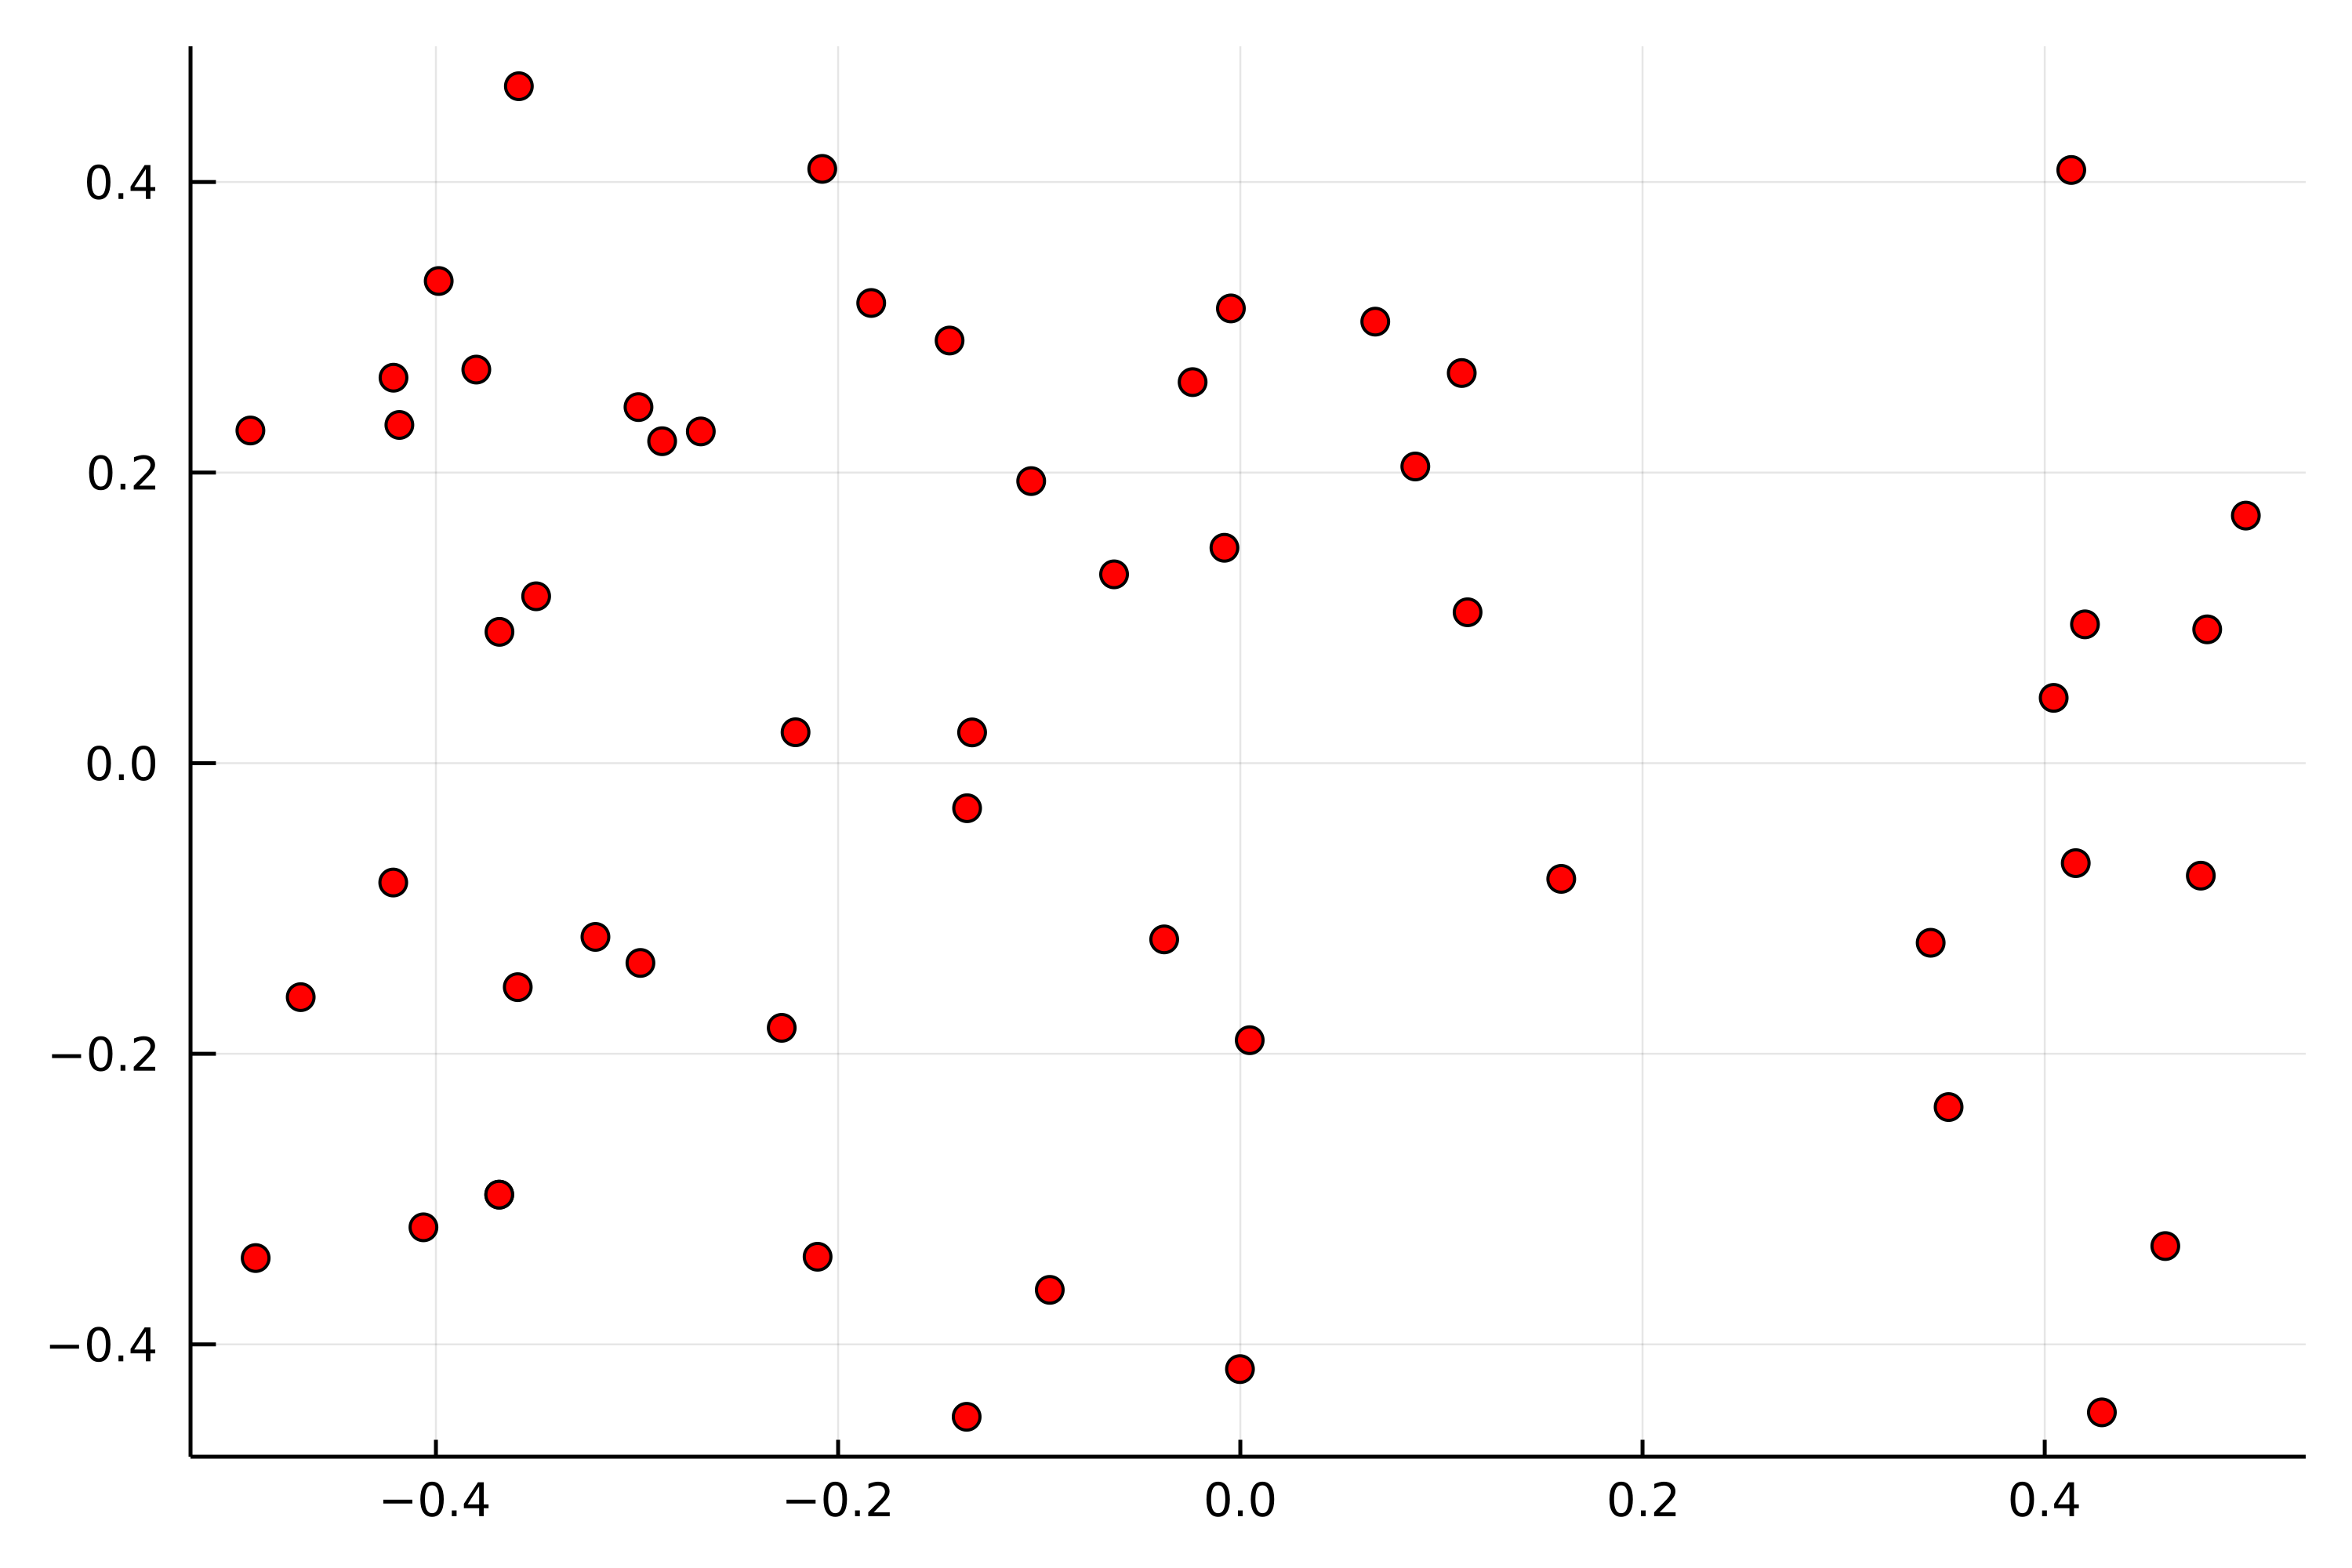
\includegraphics[width = \textwidth]{images/introduction/tourscatter}
		\caption{} 
	\end{subfigure}
	~
	\begin{subfigure}{0.5\linewidth}
		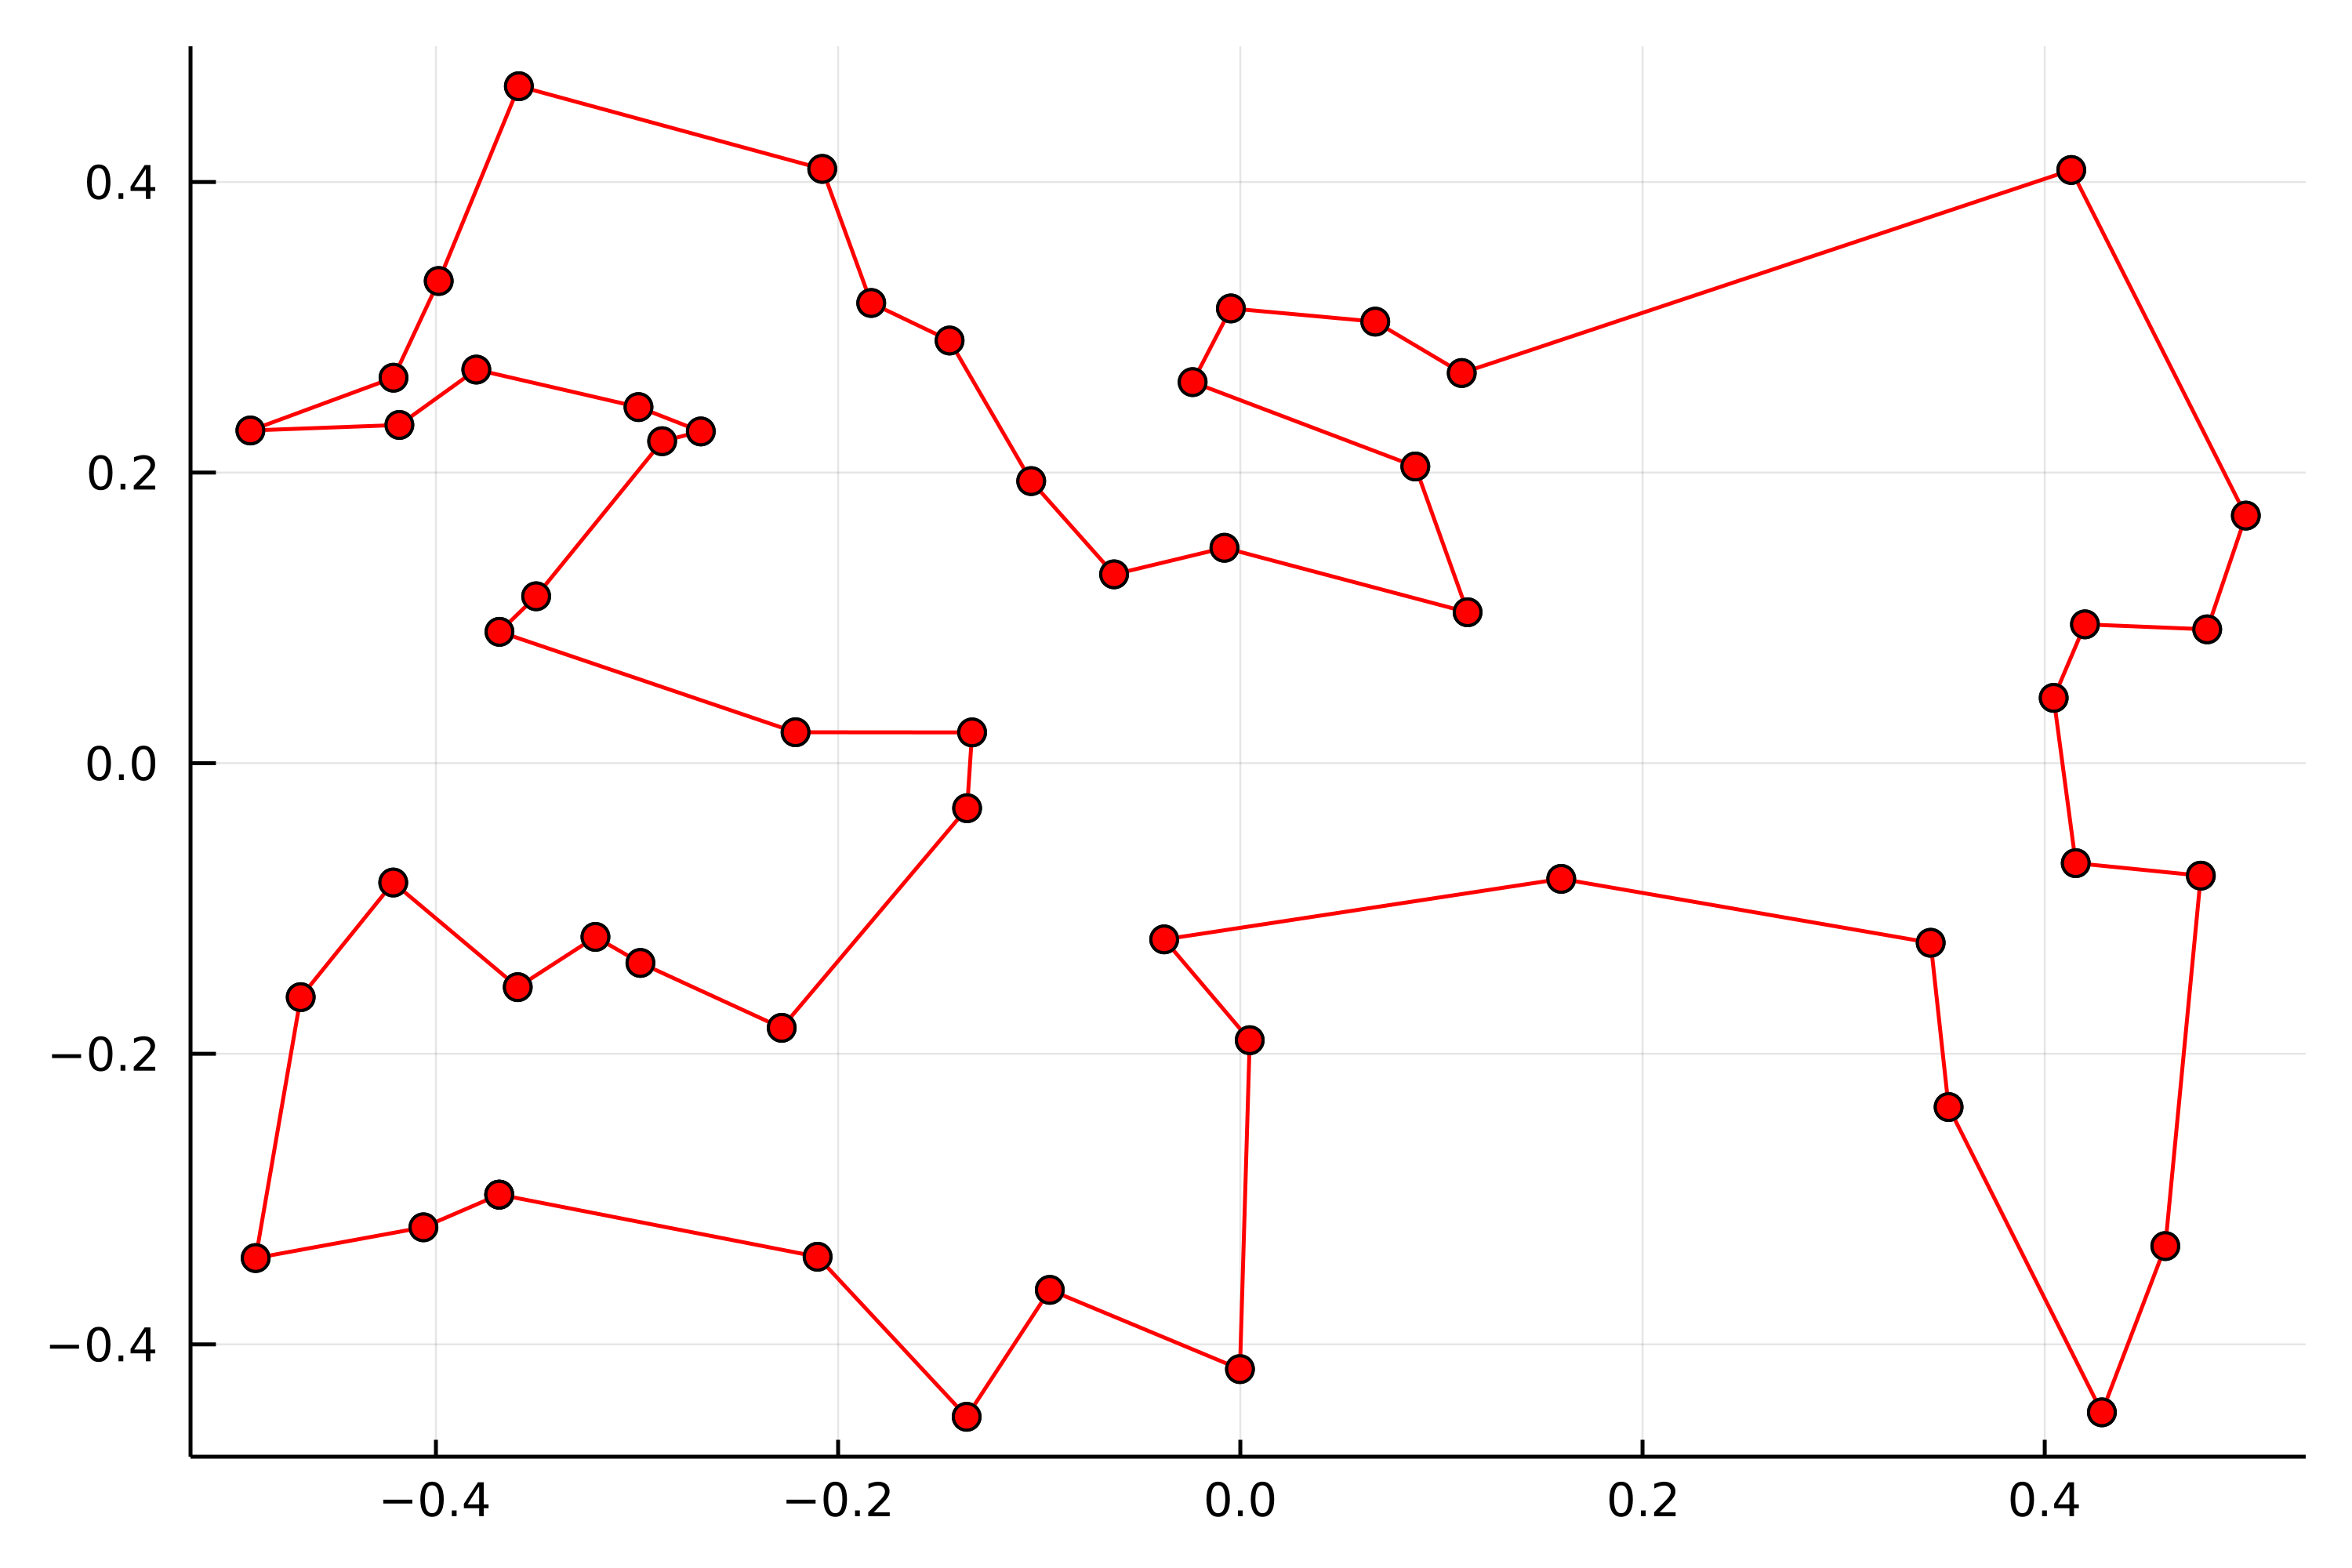
\includegraphics[width = \textwidth]{images/introduction/tourvalid}
		\caption{} 
	\end{subfigure}
	\def\c{A description of the Travelling Salesman Problem. }
	\caption[\c]{A series of nodes scattered uniformly in the unit square is shown in the left panel (a) while a valid tour passing through each of these nodes once before returning to the initial node is shown in the right panel (b). There are n! such tours and while this example does not exhibit a tour crossing they are ostensibly possible. Due to the metric triangle inequality any tour with a crossing can be improved and they are thus provably sub-optimal.}
\end{figure}

There is an interesting relationship with the TSP and topographic maps which was first introduced by the Elastic Net algorithm a heuristic designed to solve the metric Travelling Salesman which was a successor to the Tea-Trade model of retinotopic development \cite{Durbin1987-ki, Willshaw1976-ew}. The model is an energy minimisation model which deforms a net of elastic beads, where neighbours are connected elastically by spring forces, to a set of nodes which provide attractive forces to each of the beads. Supposing that there are $N$ nodes and $M$ beads and letting $X = \{\vec{x}_i : i = 1, ..., N \}$ and $Y = \{\vec{y}_i : i = 1, ..., M \}$ the energy of a given bead configuration is given by a functional parametrised by $\alpha, \beta, K$:
\begin{equation}
E[Y|X; \alpha, \beta, K] = -\alpha \sum_{i = 1}^{M} \log \left( \sum_{j=1}^N \exp\left ( \frac{- \lVert \vec{x}_i - \vec{y}_j \rVert^2 }{ 2 K^2 }  \right) \right) + \beta \sum_{j=1}^{N} \lVert \vec{y}_j - \vec{y}_{j-1} \rVert^2,
\end{equation}
In the limiting case of $K\rightarrow0$ the attractive energy provided in the first term is only significant in a small radius around each node while the tension term dominates in all other areas. The local minima of this functional in this limit are therefore straight line geodesics corresponding to the tension term that travel between each of the cities. Thus, these minima correspond to valid tours of the TSP. The functional can be minimised by gradient descent to find a local minima $K$; see Section \ref{sec:minimisation}. The gradient is calculated as:
\begin{equation}
\partial_t \vec{y}_j(t) = \beta K \left(\vec{y}_{j-1} - 2 \vec{y}_j + \vec{y}_{j+1}  \right) + \alpha \sum_{i = 1}^M (\vec{x}_i - \vec{y}_j) W(\vec{x}_i, \vec{y}_j, K(t); Y),
\end{equation}
where $W(\vec{z}_i, \vec{y}_i, K; Y) = \exp(- \lVert \vec{x}_i - \vec{y}_j \rVert^2 / (2 K^2)) / \sum_{j = 1}^N \exp(- \lVert \vec{z}_i - \vec{y}_j \rVert^2 / (2 K^2))$. This rule is applied 25 times for each $K$ after which $K$ is reduced by the mapping $K\leftarrow0.99K$. When $K$ has reached a sufficiently low value the procedure is terminated. A cartoon of this procedure can be seen in Figure \ref{fig:encartoon}.

\begin{figure}
	\centering
	\includegraphics[width=\textwidth]{images/introduction/elasticNetexample}
	\def\c{A description of the Elastic Net method for producing solutions to the Travelling Salesman Problem. }
	\caption[\c]{\label{fig:encartoon} The Elastic Net is initialised in a circle of radius 0.2 around the centre of mass of the nodes. As K is decreased exponentially and the algorithm moves through its gradient descent the beads are deformed (a-d). K must decrease sufficiently slowly to prevent edge cross-overs; an almost cross-over is shown in (c). This cross-over prevention significantly hampers algorithmic performance as there is no native penalty imposed on cross-overs. The reason decreasing K slowly ensures crossover prevention is due to a sufficiently slow descent being homotopic and thus topologically preserving winding number which must be the same as the initial circle for a tour without crosses. The final tour found by traversing the configuration in (d) is shown in (e) while the best known tour is shown in (f).  Figure adapted from Durbin and Willshaw (1987) \cite{Durbin1987-ki}}
\end{figure}

Development of the Elastic Net has focused primarily on parameter selection with analysis determining optimal rules of thumb for setting the $\alpha/\beta$ ratio and discussion about the limiting aspects of this and how they may be compensated with additional parameter manipulation such as the node-bead ratio \cite{Simmen1991-hm, Durbin1989-gs}. A variation of the Elastic Net was proposed to give substantial computational performance reducing the amount of information considered at each step with minimal performance loss \cite{Boeres1992-fo, Burr1988-fg}. As a TSP heuristic the Elastic Net has been largely superseded with the two predominant heuristics being the Lin-Kernighan heuristic (LKH) developed by Helsgaun, and an Edge-Assembly-Crossover Genetic Algorithm (EAX-GA) being the most successful and of primary interest to this work \cite{Honda2013-ri, Nagata2013-we, Lin1973-pt, Helsgaun2009-dl}. There have been many other biologically inspired heuristics with varying degrees of performance but these will not be detailed further.  

Remarkably, the Elastic Net model was then generalised and reverse engineered to generate topological feature maps: maps whereby a visual feature such as orientation selectivity is smoothly varied across the cortical sheet \cite{Bednar2016-lg}. The generalisation was made by allowing interactions between all beads in the net, not just indexed neighbours. This is an example of a bead stencil and general theory of these stencils is given by Carreira-Perpinan and Goodhill (2011) \cite{Carreira-Perpinan2011-aa}. An account of these phenomena were given by Mitchison and Durbin (1989) who argued that these could be understood in the context of the Elastic Net performing a dimension reduction onto the 2D cortical sheet. This reduction preserves continuity and critically maintains a low wiring cost suggesting that the brain evolved minimal wiring principles and the Elastic Net was one such minimisation scheme \cite{Durbin1990-tn}. The minimal wiring principle has received much attention as a guiding organisational principle \cite{Chklovskii2004-da}. The Elastic Net model was able to generate and account for orientation selectivity, retinotopy, and ocular dominance \cite{Goodhill2000-on, Goodhill1994-dn, Goodhill2000-vp, Goodhill1990-dr}. Interestingly, the introduction of the orientation variables resulted in a deformation of normal retinotopy with the map being highly concentrated around regions of rapid change in the orientation variable; see Figure. This stood as a prediction of the model but optical imaging generated maps of V1, which encodes orientation selectivity, in mice do not appear to show this distorted retinotopic representation in either bulk or phase based measurements; see Figure \ref{fig:v1retinotopy}. 
\begin{figure}
	\centering
	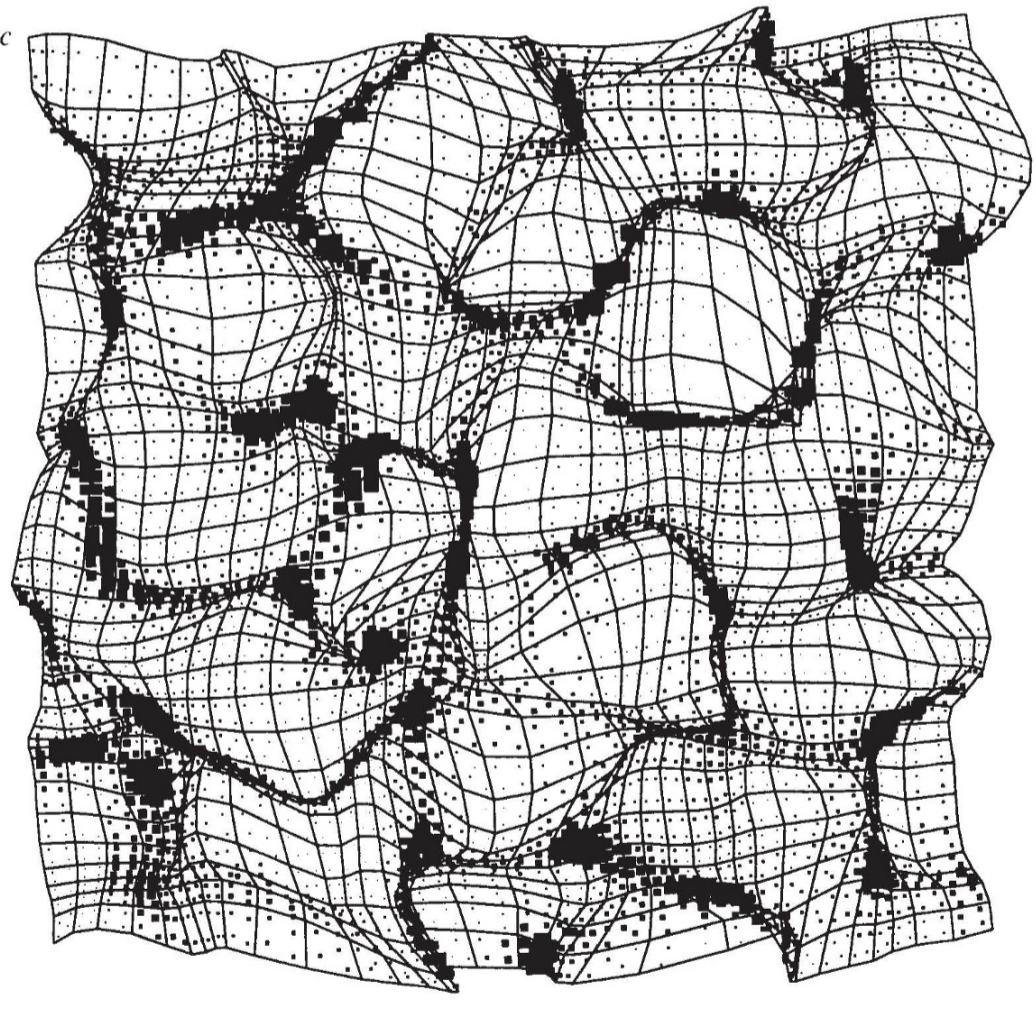
\includegraphics[width=\textwidth]{images/introduction/distortedretinotopy}
	\def\c{Prediction of retinotopy generated by the Elastic Net model when orientation curves are simultaneously trained. }
	\caption[\c]{\label{fig:distortedretinotopy} \c Trained retinotopic locations are given by the intersection of the grid and the size of the black squares indicates the rate of change of the orientation variable. Distorted retinotopic fields are generated around regions where the orientation selectivity changes most rapidly. Figure adapted from Durbin and Mitchinson (1990) \cite{Durbin1990-tn}}
\end{figure}


\begin{figure}
\centering
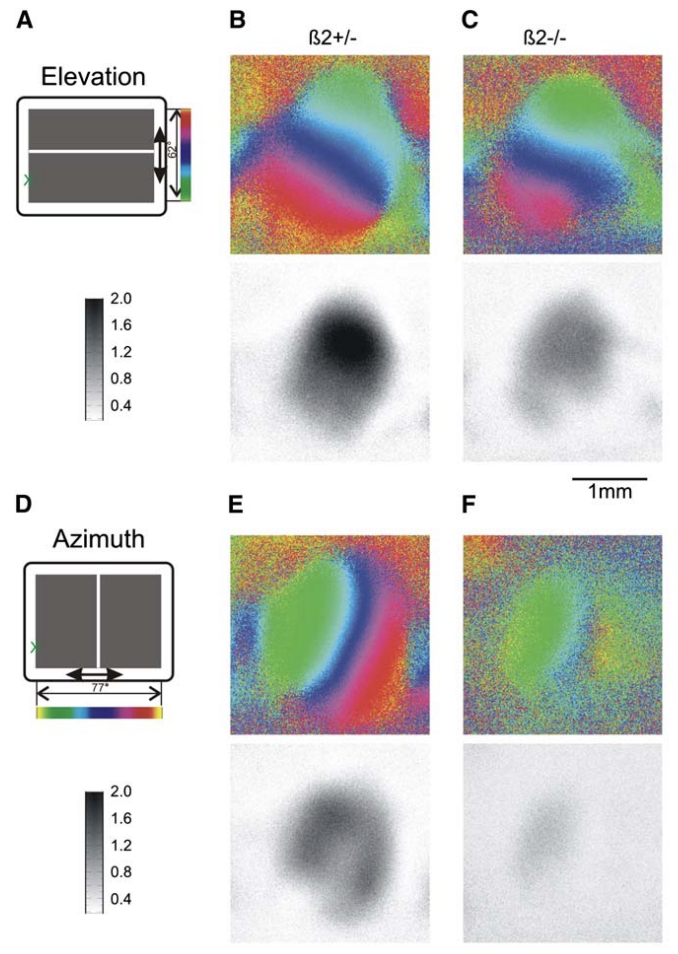
\includegraphics[width=\textwidth]{images/introduction/V1retinotopy}
\def\c{Observations of the uniformity of topographic maps formed in the retinotopic map in mice. }
\caption[\c]{\label{fig:v1retinotopy} Optical imaging scans in both azimuthal and elevational of two phenotypes of regular (B) and deficient (C) spontaneous activity patterns. In both instances the phase and bulk activity scans do not show a distorted retinotopic map. Figure adapted from Cang et. al (2005) \cite{Cang2005-eg}}
\end{figure}
\newpage
\section{Conclusions and Existing Problems}
The field of retinotopic map development has matured to the point of having relatively well understood development mechanisms and frameworks in which to embed them. There is a clear need to understand the effects of activity and in particular predict the organisational properties of the $\beta2^{-/-}$ mutant development. Key issues for the current class of unified models are parameter sensitivity and statistical analysis, and a method to link time courses in the model with developmental time courses present in biology. The understanding of development mechanisms guiding map development have matured and could be incorporated into a heuristic optimiser to aid in solving NP hard problems efficiently.
\subsection{$\beta2^{-/-}$ mutant Analysis \label{sec:beta2justification}}
The majority of recent modelling work has focused on explaining phenotypes of genetic manipulations of gradients with a particular focus on the EphA3 knock-in \cite{Savier2020-xb}. The $Math5^{-/-}$ mutant has garnered some attention but is limited due to the sparsity of available data and the modelling results only serving to confirm existing theory \cite{Triplett2011-jk, Hjorth2015-le}. An active area of experimental research is the $\beta2^{-/-}$ mutant mouse phenotype  \cite{Stafford2009, Dhande2011-jp, Chandrasekaran2005-ug, Xu2015-uc}. Despite this activity only three models have been proposed to explain the principle result: the wider arborisation of the retinal afferents. Of these three models two will be discussed because while the third claims to reproduce the phenotypic effects it offers no detail on the model construction or implementation which prohibits any meaningful interpretation \cite{Xu2011-mt}.

The GSE model uses a wider correlation function alongside an integrate-and-fire spiking model coupled with STDP to model the phenotype and found that while a wider arborisation could be predicted it was an order of magnitude larger than experimental results. It should be noted that the GSE model introduced the activity mechanism after a period of chemotactic development. When the mechanism was introduced earlier it disrupted the development of all topography. It should be noted that the GSE model is extremely computationally demanding taking on the order of five days to generate a single map. It is therefore infeasible to come to a reliable understanding of the variance in its generative mechanisms when tuning parameters to experimental data. The GSE study concluded that it was unlikely that the spatio-temporal statistics of the retinal waves played any role in the developmental process.

The second model attempted to modify the correlation functions in the Tsigankov-Koulakov formalism according to experimental data. The result was reproducing features of the wild-type maps that the model typically generates, but at a much faster rate. Since this formalism instantiates activity purely on distance-based correlations this result suggests that the spatio-temporal structure of the waves may be important, contradicting the conclusion of the previous study.

The body of experimental work suggest a keen interest in understanding the $\beta2^{-/-}$ mutant phenotype but the currently proposed models have had limited success in predicting the primary experimental result. The seeming contradiction in conclusions about the effect of spatio-temporal statistics in existing models suggest that a more detailed theoretical understanding of this aspect of the phenomenon is required. Furthermore, a model must be sufficiently lightweight in both parameter space and execution time to offer meaningful statistical comparison to available data. The development and analysis of this model will be the focus of Chapter \ref{chapter:neuralstdp}
\subsection{EphA3 Knock-In Dataset }
The dataset by Owens et al (2015) presents some interesting challenges principally in the argument or interpretation of the data. Under their interpretation the EphA3$^{+/-}$ map is driven by a stochastic process resulting in the single knock-in maps presenting occasionally as single, mixed, or double maps \cite{Owens2015-zv}. Additionally, $\beta2^{-/-}$ mutants were crossed with EphA3 knock-ins and examined. The paper suggested that these mutants presented a wild-type phenotype with slightly lower amplitudes. They thus proposed a competitive balance of molecular and activity based cues which results in map heterogeneity. 

The stochastic component of the argument is further justified by the use of an early version of the Koulakov model which the authors claim to reproduce the stochastic behaviour observed in the data. Furthermore, in this version of the Tsigankov-Koulakov model competition is implicitly defined by the requirement of a one-to-one mapping which leads naturally to interdigitating maps when chemical affinities are identical. This strict competition mechanism could thus produce maps which appear stochastic arising from the minimisation procedure, but do not represent biologically plausible maps i.e. this effect may be an artefact of the modelling. Interestingly, a modelling study using the updated version of the Tsiganov-Koulakov model were able to reproduce the $\beta2^{-/-}$EphA3$^{+/+}$, and EphA3$^{+/+}$ phenotypes lending some support to the original hypothesis. An analogous study modelling $\beta2^{-/-}$ effects in a similar way concluded that this method meant the activity effects had become dominant in the model \cite{Lyngholm2019-fs}. Activity is sufficient for unoriented topography and a model of neural activity has shown to be able to correct defects in poorly established topographic mappings with a secondary study showing the model can account for the widened arbors in the $\beta2^{-/-}$ mutant \cite{Chandrasekaran2005-ug, McLaughlin2003-yy}. Taken together, these results imply that the choice of modelling parameters resulted in a strong activity dominating any map aberrations introduced by the modified EphA3$^{+/-}$ gradient and producing the desired phenotype, but in the absence of EphA3$^{+/-}$ modelling does not imply stochastic balancing behaviour.

Preliminary unpublished analysis by David Willshaw revealed that the prevalence of stochastic seeming phenotypes might have stemmed from a miscategorised data point: a homozygote was labelled as a heterozygote. Taken in conjunction with analysis restricted to one dimension and a confounding factor in the modelling suggest that the data should be re-evaluated. To understand this dataset more thoroughly two things are essential: a revisiting of the map data analysis including all available 2D data about the map and a robust analysis method, and a modelling study of the EphA3+/- single knock-in using the updated Tsigankov-Koulakov model. Further to this, a reanalysis presents an excellent opportunity to understand the statistical properties of the Tsigankov-Koulakov model. Analysis on this dataset will be performed alongside theoretical analysis in Chapter \ref{chapter:lattice}.
\subsection{Efficient Unified Modelling \label{sec:efficientmodelling}}
A key issue of recent unified models of topographic map formation is a lack of understanding in the model parameter space and how these parameters change when considering different mutant data. The near universality of many models ensure that with sufficient parameter tweaking a desired outcome can be achieved which makes model assessment challenging. A proposed pipeline for model assessment was given by Hjorth et. al. (2015) but the problem of understanding how the parameters can be manipulated remains. These studies are limited principally because the models are computationally demanding. The only known parameter sensitivity study on the Tsigankov-Koulakov formulation required typically unobtainable amounts of super computer time \cite{Tikidji-Hamburyan2016-sn}. These make parameter fitting methods and various statistical methodologies out of reach.

Therefore, there is a pressing need to reformulate the salient features of the unified models into a computationally efficient format that does not comprise explanatory power. The most parsimonious explanations of modelling data are given by the Tsigankov-Koulakov model and therefore it seems reasonable to exploit the principle features of that model: graded matching, distance dependent correlation functions, and competition based on some polynomial function of synaptic density. The model however does not have a natural interpretation of time and relying on a stochastic minimisation procedure. The Simpson-Goodhill and GSE models fare well in this regard as their differential formulation allow a natural way to correlate the development of the model with developmental time points in the system. Fortunately, there is a natural way to reformulate energy based functional models into differential ones through the gradient descent method of functional minimisation; see Section \ref{sec:graddescent}. The development of this computationally efficient formulation shall be the subject of Chapter 4.

\subsection{Heuristics}
The Elastic Net was developed on the basis of a retinotopic map formation model and is a parallel and efficient solver for the Travelling Salesman. The Elastic Net is notable because of its reliance on metric topologies whereas most other solvers define the problem discretely. Most work on improving the Elastic Net has been either implementing routines that execute it with speed and analysing methods to choose the correct set of parameters. An open question is whether the Elastic Net methodology can be more fundamentally improved by incorporating new understandings of retinotopic map development as well as more efficient gradient descent optimisations. These improvements will be made in Chapter \ref{chapter:elastic} and the effect on heuristic performance as well as feature selectivity will be examined. 
